\documentclass[12pt,a4paper]{article}
\usepackage[utf8]{inputenc}
\usepackage[english]{babel}
\usepackage{geometry}
\usepackage{fancyhdr}
\usepackage{graphicx}
\usepackage{float}
\usepackage{tabularx}
\usepackage{longtable}
\usepackage{array}
\usepackage{booktabs}
\usepackage{multirow}
\usepackage{listings}
\usepackage{xcolor}
\usepackage{tikz}
\usepackage{forest}
\usepackage{hyperref}
\usepackage{amsmath}
\usepackage{amsfonts}
\usepackage{amssymb}
\usepackage{enumitem}
\usepackage{caption}
\usepackage{subcaption}

% Page setup
\geometry{
    left=2.5cm,
    right=2.5cm,
    top=2.5cm,
    bottom=2.5cm
}

% Header and footer
\pagestyle{fancy}
\fancyhf{}
\rhead{HIV Clinic Management System}
\lhead{Software Design Specification}
\cfoot{\thepage}
\setlength{\headheight}{14.5pt}

% Code listing style
\lstset{
    basicstyle=\ttfamily\small,
    breaklines=true,
    frame=single,
    language=Java,
    numbers=left,
    numberstyle=\tiny,
    showstringspaces=false,
    tabsize=2,
    commentstyle=\color{gray},
    keywordstyle=\color{blue},
    stringstyle=\color{red}
}

% TikZ libraries
\usetikzlibrary{shapes.geometric, arrows, positioning, fit, backgrounds}

% Define colors
\definecolor{packagecolor}{RGB}{173, 216, 230}
\definecolor{classcolor}{RGB}{255, 218, 185}
\definecolor{interfacecolor}{RGB}{221, 160, 221}

% Title page
\title{
    \vspace{-2cm}
    \Huge\textbf{HIV Clinic Management System}\\
    \vspace{1cm}
    \Large\textbf{Software Design Specification}\\
    \vspace{2cm}
    \normalsize Version 1.0
}

\author{}
\date{
    \vspace{4cm}
    – Ho Chi Minh City, January 2025 –
}

\begin{document}

\maketitle
\thispagestyle{empty}

\newpage

% Record of changes
\section*{Record of Changes}
\begin{longtable}{|p{3cm}|p{2cm}|p{3cm}|p{6cm}|}
\hline
\textbf{Date} & \textbf{A*M, D} & \textbf{In charge} & \textbf{Change Description} \\
\hline
2025-01-06 & A & KhoaDDSE196260 & Initial creation of SDS document \\
\hline
2025-01-06 & A,M & AnPPSE196260 & Added comprehensive system architecture \\
\hline
2025-01-06 & A,M & TuanTMSE192397 & Added detailed class diagrams and specifications \\
\hline
2025-01-06 & A,M & DatNTSE194083 & Added database design and API documentation \\
\hline
\end{longtable}

\footnotesize{*A - Added, M - Modified, D - Deleted}

\newpage

% Table of contents
\tableofcontents

\newpage

\section{Overview}

\subsection{Code Packages}

The HIV Clinic Management System follows a layered architecture pattern with clear separation of concerns. The backend is built using Spring Boot framework with Java 17, while the frontend uses React with modern JavaScript (ES6+). The system implements a comprehensive package structure that promotes maintainability and scalability.

\begin{figure}[H]
\centering
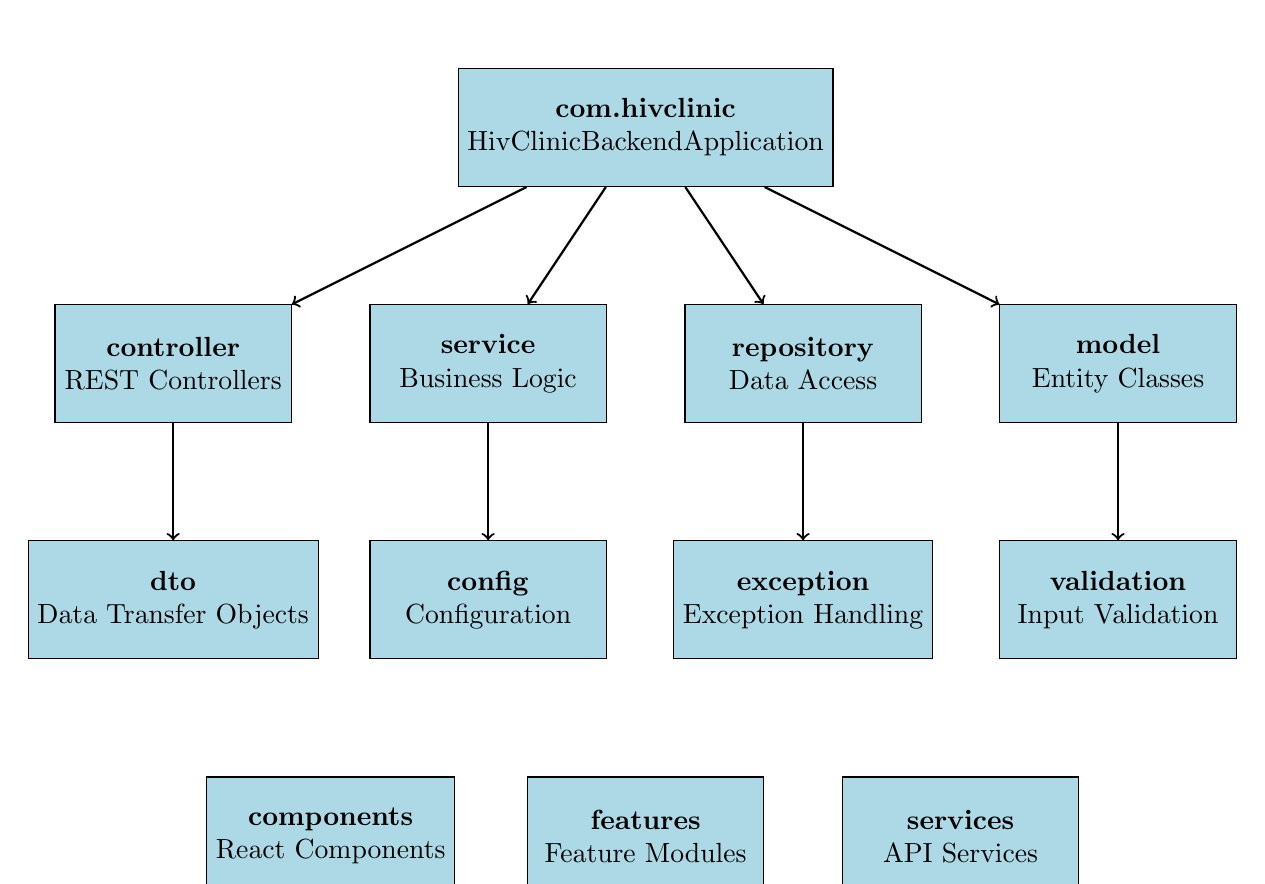
\begin{tikzpicture}[
    package/.style={draw, fill=packagecolor, minimum width=3cm, minimum height=1.5cm, text centered, align=center},
    arrow/.style={->, thick}
]

% Main application package
\node[package] (main) at (0, 0) {\textbf{com.hivclinic}\\ HivClinicBackendApplication};

% Layer packages
\node[package] (controller) at (-6, -3) {\textbf{controller}\\ REST Controllers};
\node[package] (service) at (-2, -3) {\textbf{service}\\ Business Logic};
\node[package] (repository) at (2, -3) {\textbf{repository}\\ Data Access};
\node[package] (model) at (6, -3) {\textbf{model}\\ Entity Classes};

% Supporting packages
\node[package] (dto) at (-6, -6) {\textbf{dto}\\ Data Transfer Objects};
\node[package] (config) at (-2, -6) {\textbf{config}\\ Configuration};
\node[package] (exception) at (2, -6) {\textbf{exception}\\ Exception Handling};
\node[package] (validation) at (6, -6) {\textbf{validation}\\ Input Validation};

% Frontend packages
\node[package] (components) at (-4, -9) {\textbf{components}\\ React Components};
\node[package] (features) at (0, -9) {\textbf{features}\\ Feature Modules};
\node[package] (services) at (4, -9) {\textbf{services}\\ API Services};

% Arrows
\draw[arrow] (main) -- (controller);
\draw[arrow] (main) -- (service);
\draw[arrow] (main) -- (repository);
\draw[arrow] (main) -- (model);

\draw[arrow] (controller) -- (dto);
\draw[arrow] (service) -- (config);
\draw[arrow] (repository) -- (exception);
\draw[arrow] (model) -- (validation);

\end{tikzpicture}
\caption{Package Structure Overview}
\label{fig:package-structure}
\end{figure}

\begin{table}[H]
\centering
\caption{Package Descriptions}
\label{tab:package-descriptions}
\begin{tabularx}{\textwidth}{|c|l|X|}
\hline
\textbf{No} & \textbf{Package} & \textbf{Description} \\
\hline
01 & com.hivclinic.controller & REST API endpoints handling HTTP requests and responses. Contains controllers for authentication, appointments, user management, and ARV treatments. \\
\hline
02 & com.hivclinic.service & Business logic layer implementing core application functionality. Handles appointment scheduling, notification management, and user authentication. \\
\hline
03 & com.hivclinic.repository & Data access layer using Spring Data JPA. Provides database operations for all entity classes with custom queries for complex operations. \\
\hline
04 & com.hivclinic.model & JPA entity classes representing database tables. Includes User, Appointment, ARVTreatment, Notification, and related entities. \\
\hline
05 & com.hivclinic.dto & Data Transfer Objects for API communication. Separate request and response DTOs for clean API contracts. \\
\hline
06 & com.hivclinic.config & Spring configuration classes including security, JWT, CORS, and database configuration. \\
\hline
07 & com.hivclinic.exception & Custom exception classes and global exception handling for consistent error responses. \\
\hline
08 & com.hivclinic.validation & Custom validation annotations and validators for input validation. \\
\hline
09 & components & React components organized by functionality: layout, notifications, scheduling, and ARV treatment management. \\
\hline
10 & features & Feature-based React modules for Admin, Doctor, Patient, and Manager dashboards. \\
\hline
11 & services & Frontend API service layer for HTTP communication with the backend REST API. \\
\hline
\end{tabularx}
\end{table}

\subsection{Database Design}

\subsubsection{Database Schema}

The HIV Clinic Management System uses Microsoft SQL Server as the primary database. The schema follows 3rd Normal Form (3NF) design principles with proper referential integrity constraints.

\begin{figure}[H]
\centering
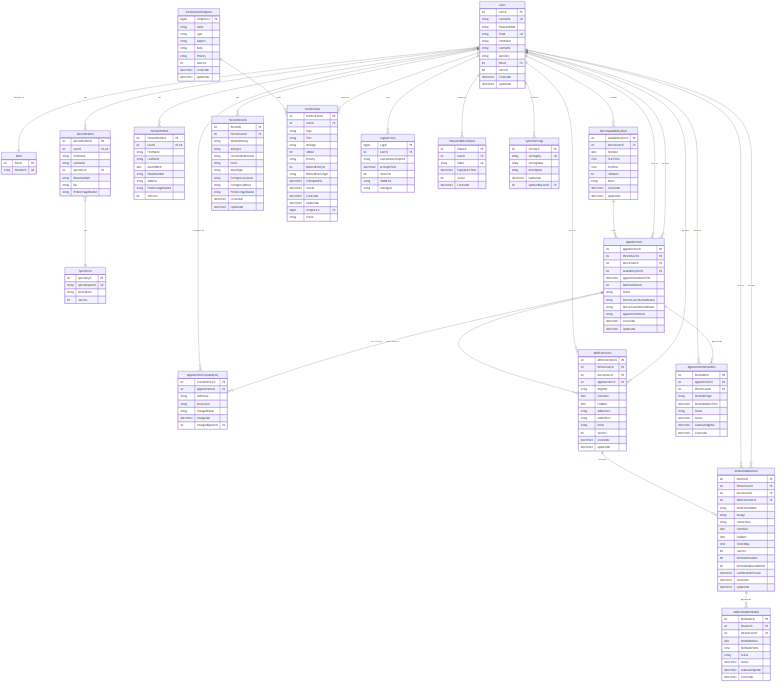
\includegraphics[width=0.9\textwidth]{diagrams/database_schema_erd.png}
\caption{Database Entity Relationship Diagram}
\label{fig:database-schema}
\end{figure}

\subsubsection{Table Description}

\begin{longtable}{|c|l|p{8cm}|}
\hline
\textbf{No} & \textbf{Table} & \textbf{Description} \\
\hline
01 & Users & Core user table storing authentication credentials and basic user information for all user types (Admin, Manager, Doctor, Patient) \\
\hline
02 & Roles & Role-based access control definitions with hierarchical permissions (Admin > Manager > Doctor > Patient) \\
\hline
03 & DoctorProfiles & Extended profile information for doctor users including specialties, bio, and profile images \\
\hline
04 & PatientProfiles & Extended profile information for patient users including demographics and privacy settings \\
\hline
05 & Specialties & Medical specialties reference table for categorizing doctors \\
\hline
06 & DoctorAvailabilitySlots & Doctor's available time slots for appointment booking with date, time, and booking status \\
\hline
07 & Appointments & Appointment records linking patients and doctors with scheduling and status information \\
\hline
08 & PatientRecords & Comprehensive medical records including history, allergies, medications, and emergency contacts \\
\hline
09 & ARVTreatments & Antiretroviral treatment records with regimen details, adherence tracking, and side effects \\
\hline
10 & Notifications & System notifications for appointment reminders, medication alerts, and general communications \\
\hline
11 & NotificationTemplates & Reusable notification templates for different notification types with customizable content \\
\hline
12 & MedicationRoutines & Daily medication schedules for patients with reminder settings and timing \\
\hline
13 & MedicationReminders & Individual medication reminder instances with status tracking \\
\hline
14 & AppointmentReminders & Appointment reminder instances with multiple reminder types (24h, 1h, 30min) \\
\hline
15 & AppointmentStatusHistory & Audit trail for appointment status changes with timestamps and reasons \\
\hline
16 & LoginActivity & Security audit log for user authentication attempts and session management \\
\hline
17 & PasswordResetTokens & Secure password reset token management with expiration and usage tracking \\
\hline
18 & SystemSettings & Configurable system parameters for application behavior and feature flags \\
\hline
\end{longtable}

\section{Code Designs}

\subsection{User Authentication and Authorization}

This section details the comprehensive authentication and authorization system implemented using Spring Security with JWT tokens.

\subsubsection{Class Diagram}

\begin{figure}[H]
\centering
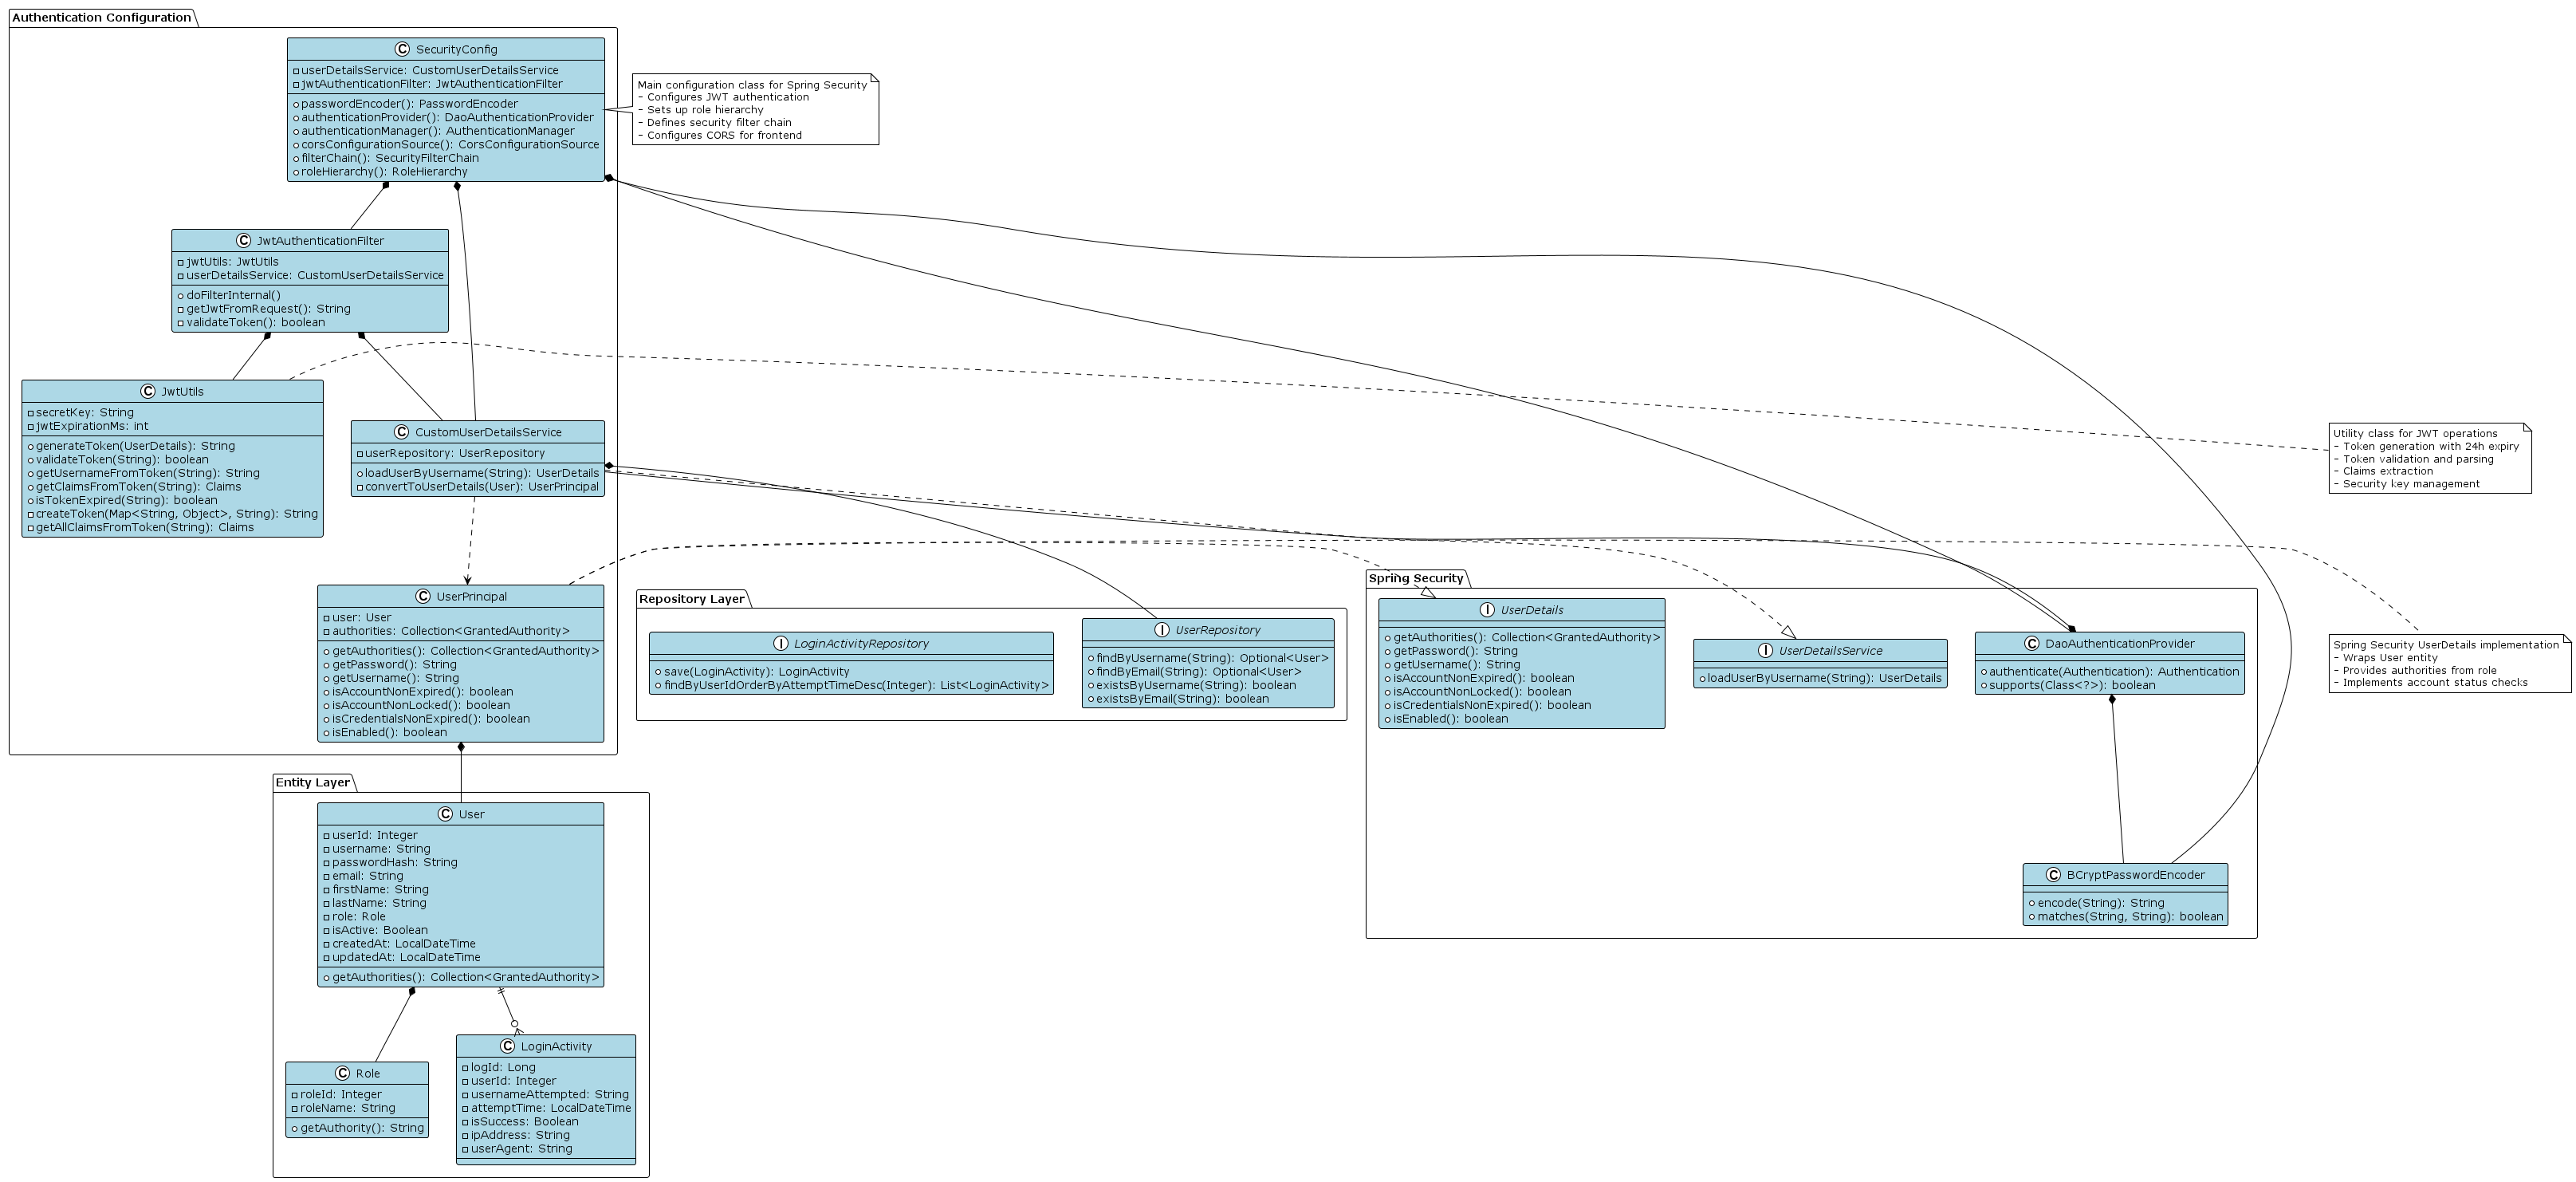
\includegraphics[width=0.9\textwidth]{diagrams/authentication_class_diagram.png}
\caption{Authentication System Class Diagram}
\label{fig:auth-class-diagram}
\end{figure}

\subsubsection{Class Specifications}

\paragraph{SecurityConfig Class}
\begin{longtable}{|c|l|p{8cm}|}
\hline
\textbf{No} & \textbf{Method} & \textbf{Description} \\
\hline
01 & passwordEncoder() & Returns BCryptPasswordEncoder instance for secure password hashing with salt \\
\hline
02 & authenticationProvider() & Configures DaoAuthenticationProvider with custom UserDetailsService and password encoder \\
\hline
03 & authenticationManager() & Provides AuthenticationManager bean for handling authentication requests \\
\hline
04 & corsConfigurationSource() & Configures CORS settings to allow cross-origin requests from frontend applications \\
\hline
05 & filterChain() & Defines security filter chain with JWT authentication, role-based access control, and endpoint security \\
\hline
06 & roleHierarchy() & Establishes role hierarchy: ADMIN > MANAGER > DOCTOR > PATIENT \\
\hline
\end{longtable}

\paragraph{JwtUtils Class}
\begin{longtable}{|c|l|p{8cm}|}
\hline
\textbf{No} & \textbf{Method} & \textbf{Description} \\
\hline
01 & generateToken() & Generates JWT token with user details, roles, and expiration time (24 hours) \\
\hline
02 & validateToken() & Validates JWT token signature, expiration, and claims integrity \\
\hline
03 & getUsernameFromToken() & Extracts username from JWT token claims for authentication \\
\hline
04 & getClaimsFromToken() & Extracts all claims from JWT token for authorization decisions \\
\hline
05 & isTokenExpired() & Checks if JWT token has expired based on expiration claim \\
\hline
\end{longtable}

\paragraph{CustomUserDetailsService Class}
\begin{longtable}{|c|l|p{8cm}|}
\hline
\textbf{No} & \textbf{Method} & \textbf{Description} \\
\hline
01 & loadUserByUsername() & Loads user details from database by username for Spring Security authentication \\
\hline
02 & UserPrincipal() & Inner class implementing UserDetails interface with user information and authorities \\
\hline
03 & getAuthorities() & Returns granted authorities based on user role for authorization \\
\hline
04 & isAccountNonExpired() & Returns account expiration status based on user active status \\
\hline
05 & isAccountNonLocked() & Returns account lock status for security purposes \\
\hline
06 & isCredentialsNonExpired() & Returns credential expiration status \\
\hline
07 & isEnabled() & Returns user enabled status based on isActive flag \\
\hline
\end{longtable}

\subsubsection{Sequence Diagram}

\begin{figure}[H]
\centering
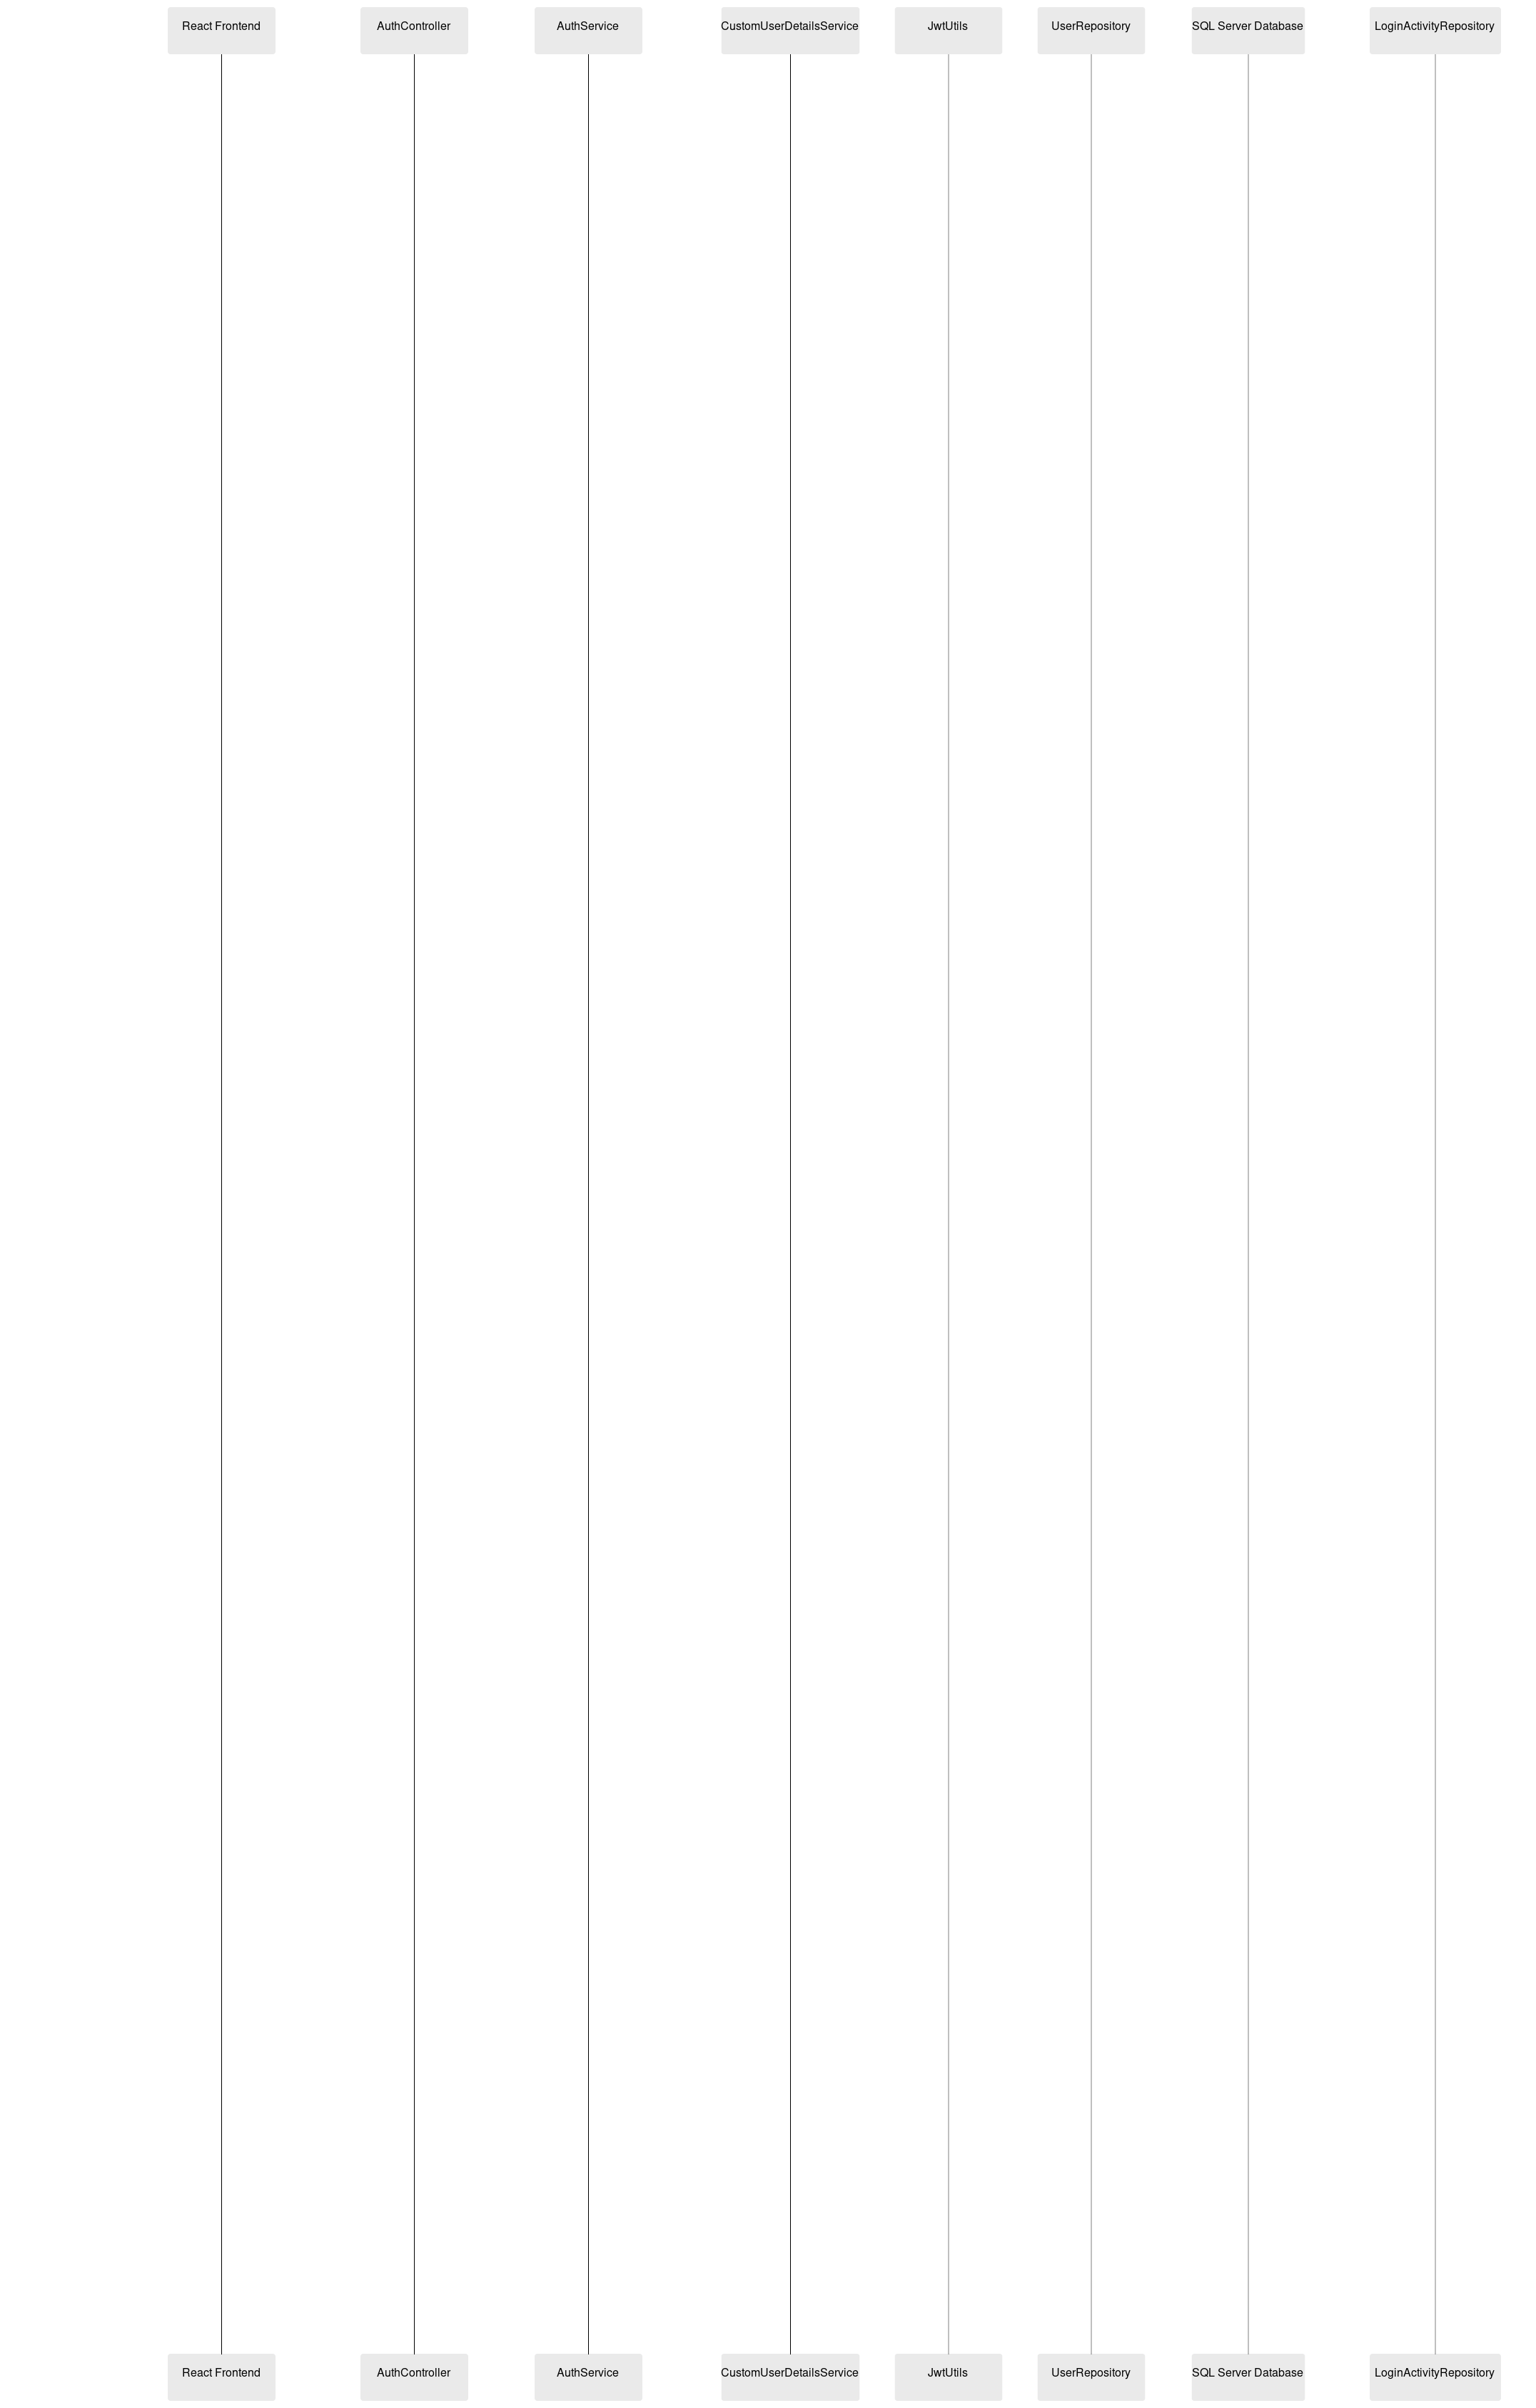
\includegraphics[width=0.9\textwidth]{diagrams/authentication_sequence.png}
\caption{Authentication Sequence Diagram}
\label{fig:auth-sequence}
\end{figure}

\subsubsection{Database Queries}

\begin{lstlisting}[language=SQL, caption=User Authentication Queries]
-- User login validation
SELECT u.UserID, u.Username, u.PasswordHash, u.Email, u.FirstName, u.LastName, 
       u.IsActive, r.RoleName
FROM Users u
INNER JOIN Roles r ON u.RoleID = r.RoleID
WHERE u.Username = ? AND u.IsActive = 1;

-- Record login activity
INSERT INTO LoginActivity (UserID, UsernameAttempted, IsSuccess, IPAddress, UserAgent)
VALUES (?, ?, ?, ?, ?);

-- Update last login timestamp
UPDATE Users SET UpdatedAt = GETDATE() WHERE UserID = ?;

-- Password reset token generation
INSERT INTO PasswordResetTokens (UserID, Token, ExpiryDateTime)
VALUES (?, ?, DATEADD(hour, 24, GETDATE()));
\end{lstlisting}

\subsection{Appointment Management System}

This section details the comprehensive appointment booking and management system.

\subsubsection{Class Diagram}

\begin{figure}[H]
\centering
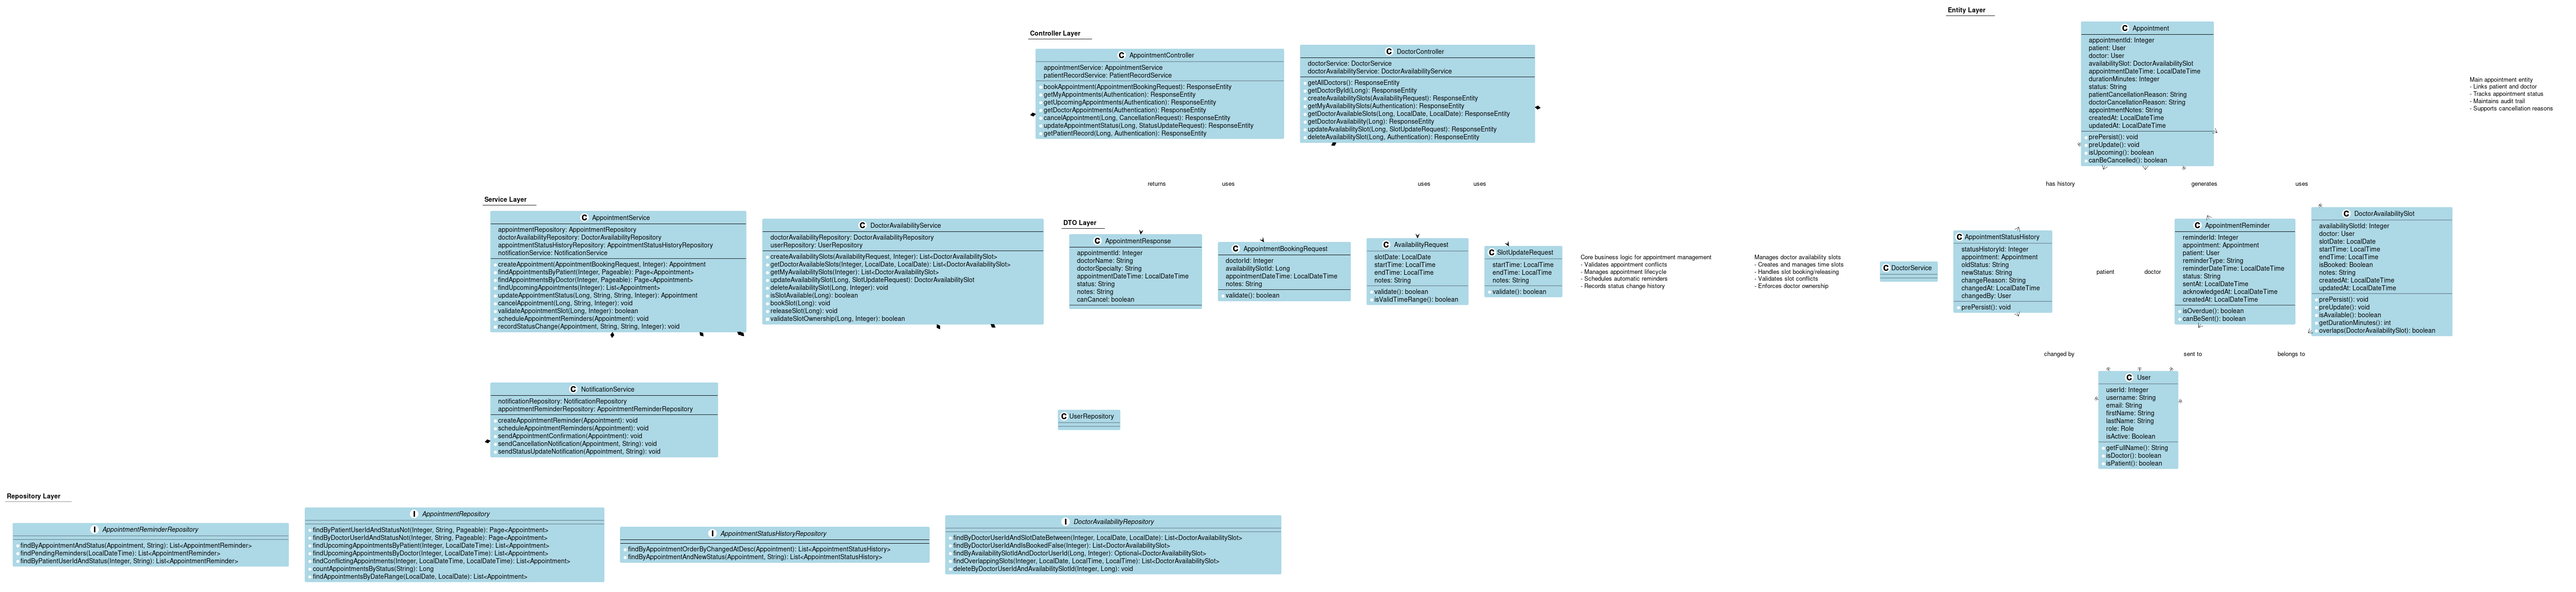
\includegraphics[width=0.9\textwidth]{diagrams/appointment_class_diagram.png}
\caption{Appointment Management Class Diagram}
\label{fig:appointment-class-diagram}
\end{figure}

\subsubsection{Class Specifications}

\paragraph{AppointmentController Class}
\begin{longtable}{|c|l|p{8cm}|}
\hline
\textbf{No} & \textbf{Method} & \textbf{Description} \\
\hline
01 & bookAppointment() & POST /api/appointments/book - Creates new appointment with patient, doctor, and time slot validation \\
\hline
02 & getMyAppointments() & GET /api/appointments/patient/my-appointments - Retrieves all appointments for authenticated patient \\
\hline
03 & getUpcomingAppointments() & GET /api/appointments/patient/upcoming - Retrieves upcoming appointments for patient dashboard \\
\hline
04 & getDoctorAppointments() & GET /api/appointments/doctor/my-appointments - Retrieves appointments for authenticated doctor \\
\hline
05 & cancelAppointment() & PUT /api/appointments/\{id\}/cancel - Cancels appointment with reason and status update \\
\hline
06 & updateAppointmentStatus() & PUT /api/appointments/\{id\}/status - Updates appointment status (Completed, No-show, etc.) \\
\hline
07 & getPatientRecord() & GET /api/appointments/\{id\}/patient-record - Retrieves patient record for appointment context \\
\hline
\end{longtable}

\paragraph{AppointmentService Class}
\begin{longtable}{|c|l|p{8cm}|}
\hline
\textbf{No} & \textbf{Method} & \textbf{Description} \\
\hline
01 & createAppointment() & Creates new appointment with slot validation, conflict checking, and notification scheduling \\
\hline
02 & findAppointmentsByPatient() & Retrieves appointments for specific patient with filtering and pagination \\
\hline
03 & findAppointmentsByDoctor() & Retrieves appointments for specific doctor with date range filtering \\
\hline
04 & updateAppointmentStatus() & Updates appointment status with history tracking and notification triggers \\
\hline
05 & cancelAppointment() & Cancels appointment, frees time slot, and sends cancellation notifications \\
\hline
06 & validateAppointmentSlot() & Validates time slot availability and conflicts before booking \\
\hline
07 & scheduleAppointmentReminders() & Schedules automatic reminders (24h, 1h, 30min before appointment) \\
\hline
\end{longtable}

\paragraph{Appointment Entity Class}
\begin{longtable}{|c|l|p{8cm}|}
\hline
\textbf{No} & \textbf{Method/Field} & \textbf{Description} \\
\hline
01 & appointmentId & Primary key with auto-increment identity \\
\hline
02 & patientUserID & Foreign key reference to Users table for patient \\
\hline
03 & doctorUserID & Foreign key reference to Users table for doctor \\
\hline
04 & availabilitySlotID & Foreign key reference to DoctorAvailabilitySlots table \\
\hline
05 & appointmentDateTime & Scheduled date and time for the appointment \\
\hline
06 & status & Current appointment status (Scheduled, Completed, Cancelled, No-show) \\
\hline
07 & appointmentNotes & Notes and comments from doctor or patient \\
\hline
08 & prePersist() & Sets creation timestamp before entity persistence \\
\hline
09 & preUpdate() & Updates modification timestamp before entity update \\
\hline
\end{longtable}

\subsubsection{Sequence Diagram}

\begin{figure}[H]
\centering
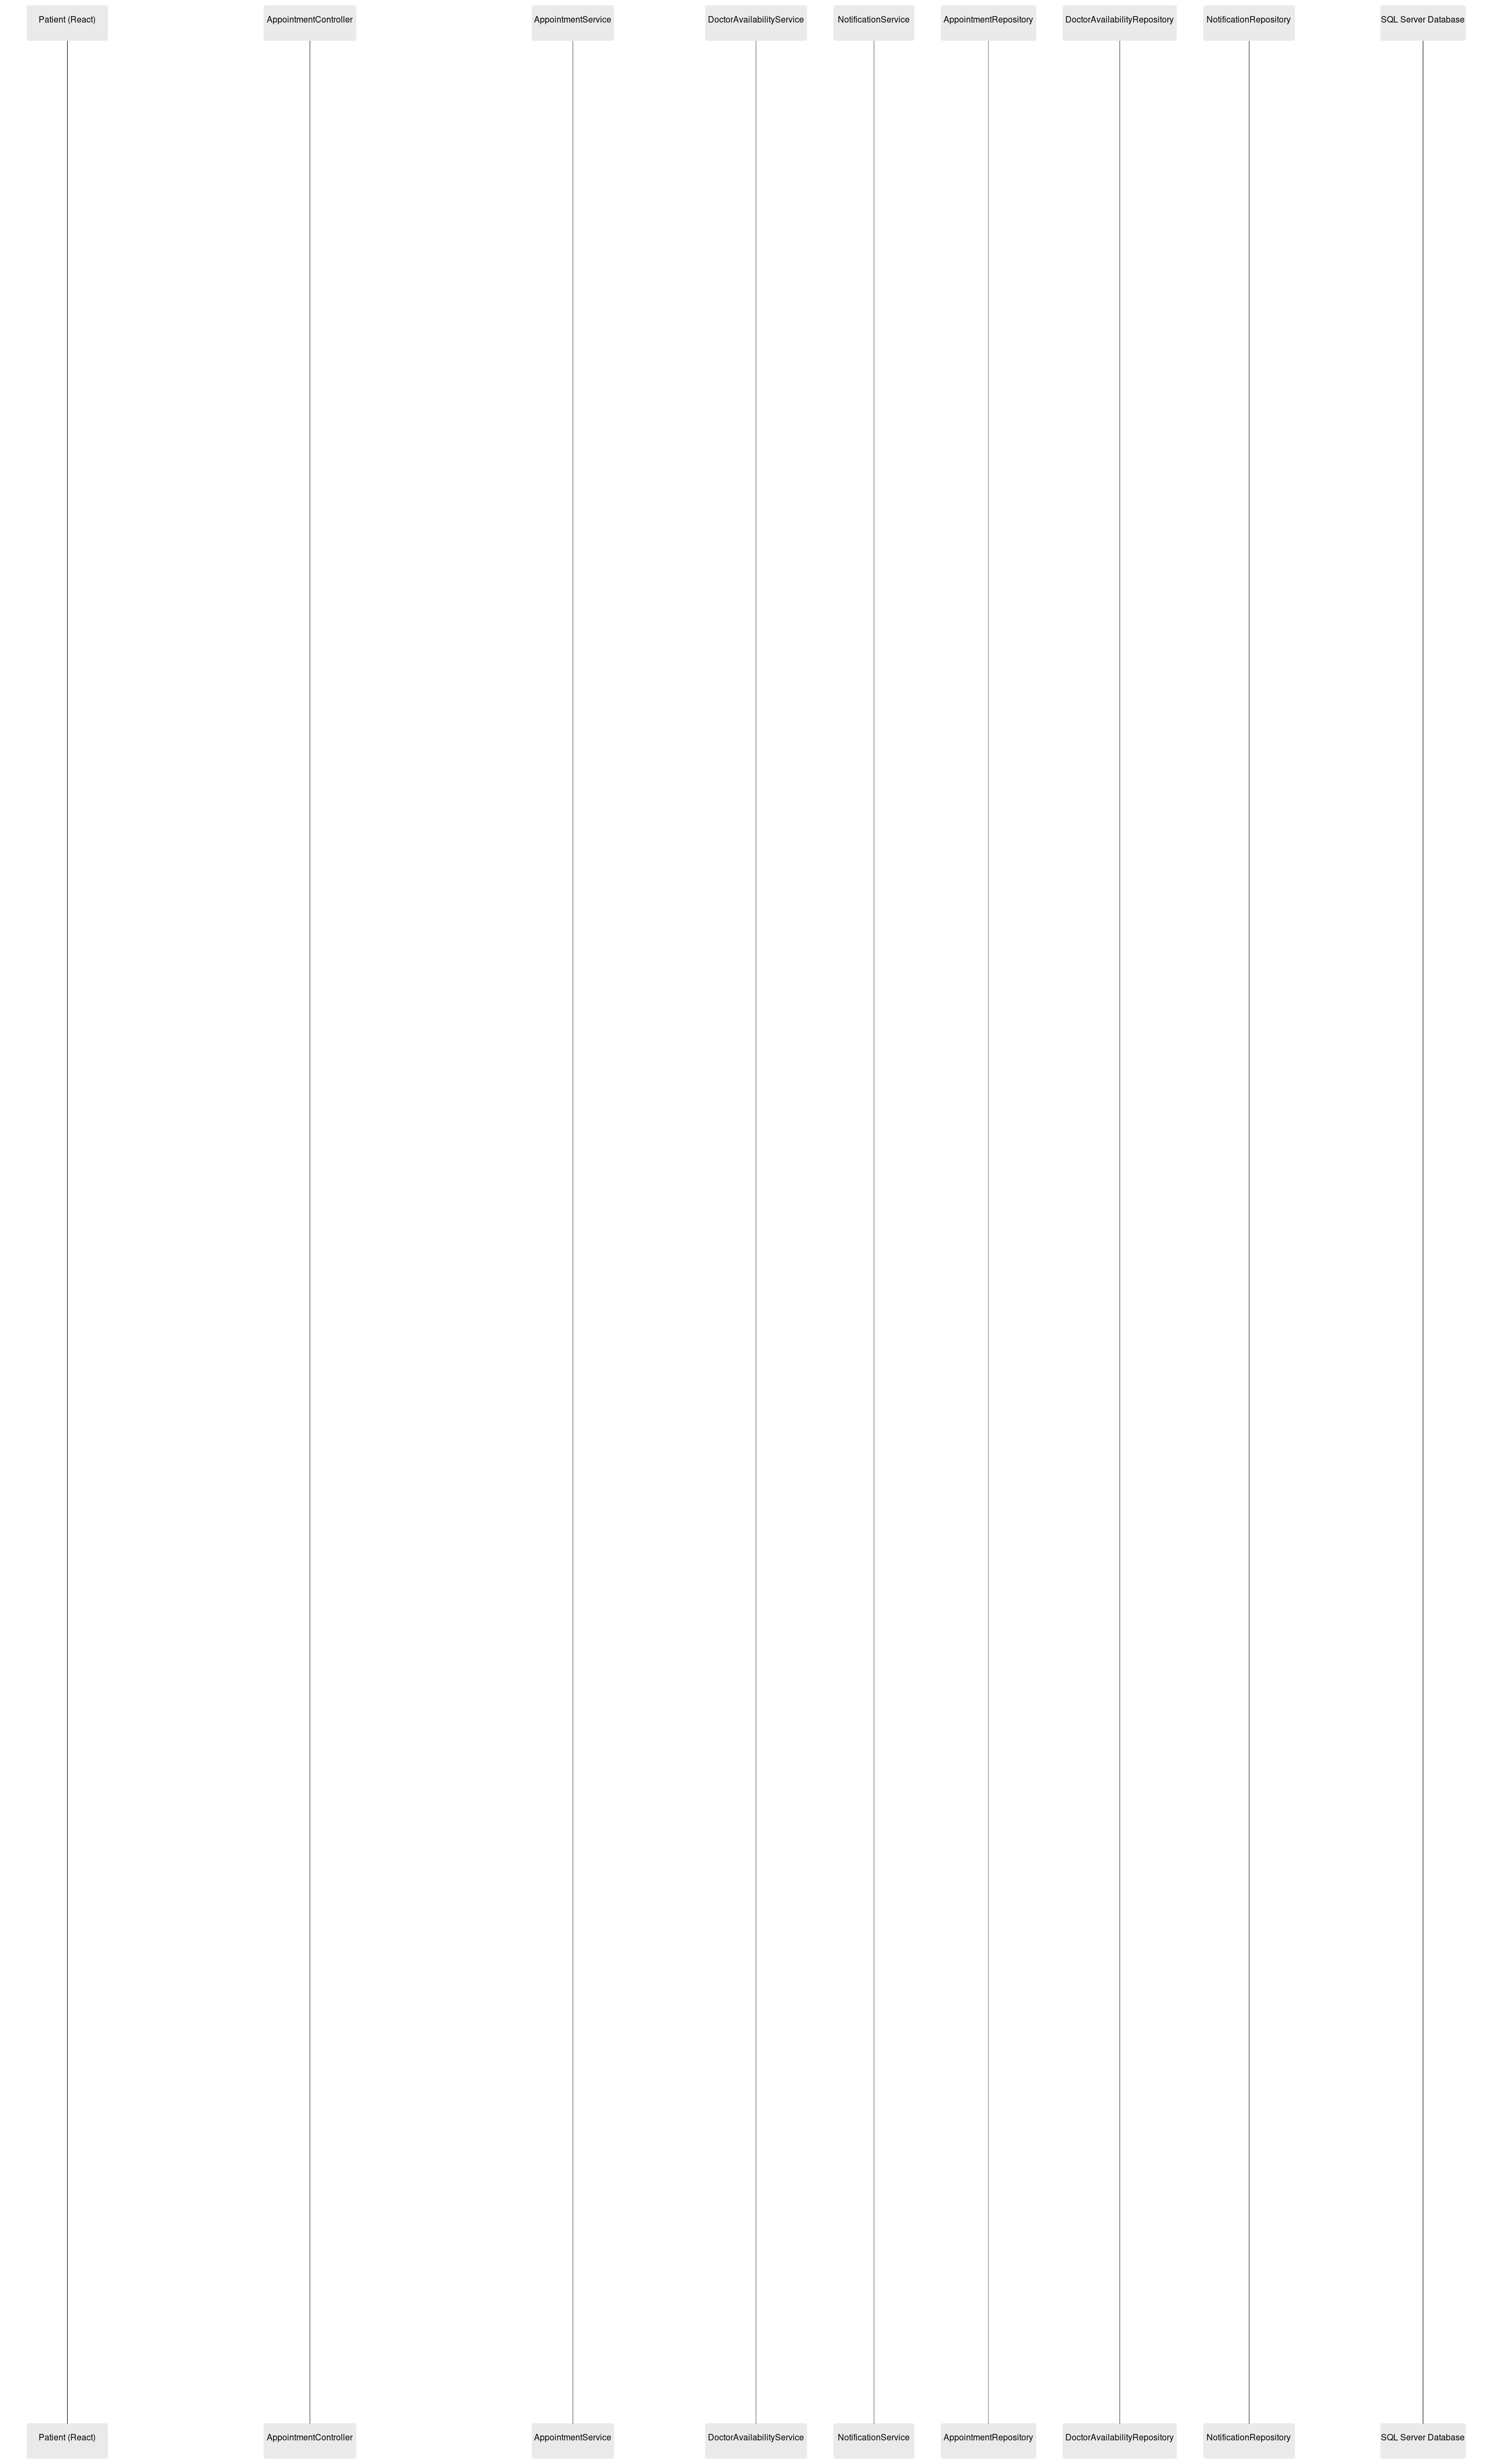
\includegraphics[width=0.9\textwidth]{diagrams/appointment_booking_sequence.png}
\caption{Appointment Booking Sequence Diagram}
\label{fig:appointment-sequence}
\end{figure}

\subsubsection{Database Queries}

\begin{lstlisting}[language=SQL, caption=Appointment Management Queries]
-- Create new appointment
INSERT INTO Appointments (PatientUserID, DoctorUserID, AvailabilitySlotID, 
                         AppointmentDateTime, Status, AppointmentNotes)
VALUES (?, ?, ?, ?, 'Scheduled', ?);

-- Update availability slot as booked
UPDATE DoctorAvailabilitySlots 
SET IsBooked = 1, UpdatedAt = GETDATE() 
WHERE AvailabilitySlotID = ?;

-- Get patient appointments with doctor details
SELECT a.*, d.FirstName as DoctorFirstName, d.LastName as DoctorLastName, 
       s.SpecialtyName, das.SlotDate, das.StartTime, das.EndTime
FROM Appointments a
INNER JOIN Users du ON a.DoctorUserID = du.UserID
INNER JOIN DoctorProfiles d ON du.UserID = d.UserID
LEFT JOIN Specialties s ON d.SpecialtyID = s.SpecialtyID
LEFT JOIN DoctorAvailabilitySlots das ON a.AvailabilitySlotID = das.AvailabilitySlotID
WHERE a.PatientUserID = ? AND a.Status != 'Cancelled'
ORDER BY a.AppointmentDateTime DESC;

-- Cancel appointment and free slot
UPDATE Appointments 
SET Status = 'Cancelled', PatientCancellationReason = ?, UpdatedAt = GETDATE()
WHERE AppointmentID = ?;

UPDATE DoctorAvailabilitySlots 
SET IsBooked = 0, UpdatedAt = GETDATE() 
WHERE AvailabilitySlotID = (SELECT AvailabilitySlotID FROM Appointments WHERE AppointmentID = ?);

-- Record status change history
INSERT INTO AppointmentStatusHistory (AppointmentID, OldStatus, NewStatus, ChangeReason, ChangedByUserID)
VALUES (?, ?, ?, ?, ?);
\end{lstlisting}

\subsection{Notification Management System}

This section details the comprehensive notification system for appointment reminders, medication alerts, and general communications.

\subsubsection{Class Diagram}

\begin{figure}[H]
\centering
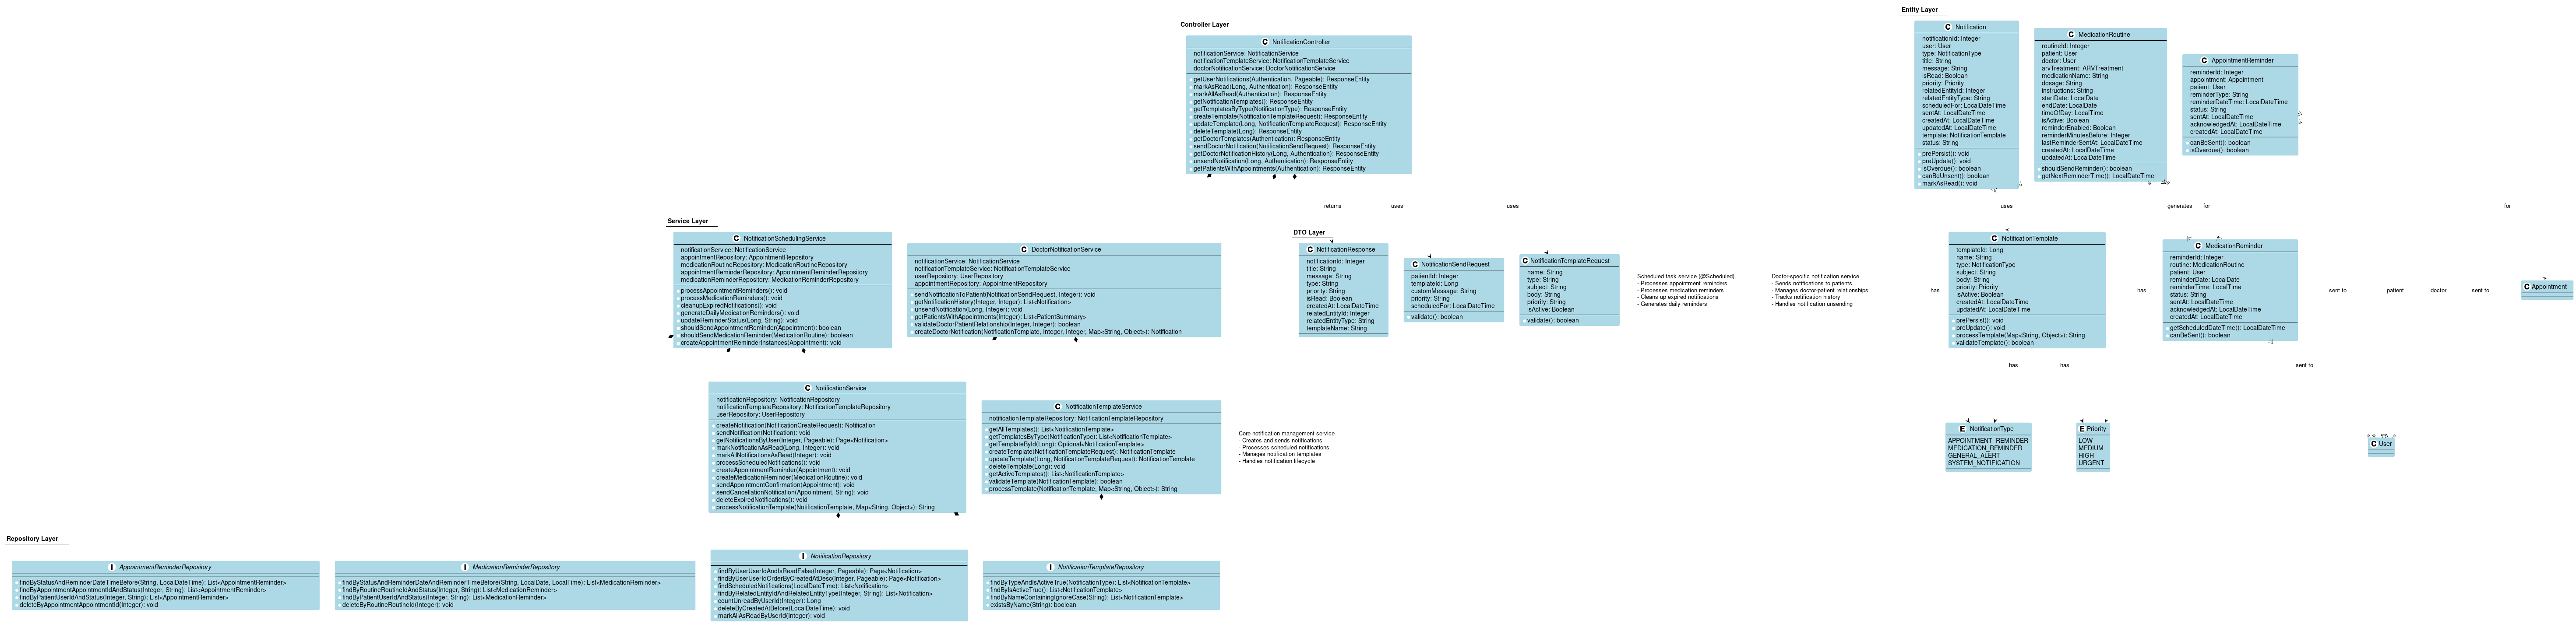
\includegraphics[width=0.9\textwidth]{diagrams/notification_class_diagram.png}
\caption{Notification System Class Diagram}
\label{fig:notification-class-diagram}
\end{figure}

\subsubsection{Class Specifications}

\paragraph{NotificationController Class}
\begin{longtable}{|c|l|p{8cm}|}
\hline
\textbf{No} & \textbf{Method} & \textbf{Description} \\
\hline
01 & getUserNotifications() & GET /api/notifications - Retrieves paginated notifications for authenticated user \\
\hline
02 & markAsRead() & POST /api/notifications/\{id\}/read - Marks specific notification as read \\
\hline
03 & markAllAsRead() & POST /api/notifications/read-all - Marks all user notifications as read \\
\hline
04 & getNotificationTemplates() & GET /api/notifications/templates - Retrieves available notification templates \\
\hline
05 & getTemplatesByType() & GET /api/notifications/templates/\{type\} - Retrieves templates by notification type \\
\hline
06 & createTemplate() & POST /api/notifications/templates - Creates new notification template \\
\hline
07 & updateTemplate() & PUT /api/notifications/templates/\{id\} - Updates existing notification template \\
\hline
08 & deleteTemplate() & DELETE /api/notifications/templates/\{id\} - Deletes notification template \\
\hline
09 & sendDoctorNotification() & POST /api/notifications/doctor/send - Sends notification from doctor to patient \\
\hline
10 & getDoctorNotificationHistory() & GET /api/notifications/doctor/history/\{patientId\} - Retrieves notification history \\
\hline
\end{longtable}

\paragraph{NotificationService Class}
\begin{longtable}{|c|l|p{8cm}|}
\hline
\textbf{No} & \textbf{Method} & \textbf{Description} \\
\hline
01 & createNotification() & Creates new notification with template processing and scheduling \\
\hline
02 & sendNotification() & Sends notification to user with delivery tracking \\
\hline
03 & scheduleAppointmentReminders() & Schedules automatic appointment reminders (24h, 1h, 30min) \\
\hline
04 & scheduleMedicationReminders() & Schedules daily medication reminders based on routines \\
\hline
05 & processScheduledNotifications() & Processes pending notifications scheduled for delivery \\
\hline
06 & markNotificationAsRead() & Marks notification as read and updates timestamp \\
\hline
07 & getNotificationsByUser() & Retrieves paginated notifications for specific user \\
\hline
08 & deleteExpiredNotifications() & Cleanup job for removing old notifications \\
\hline
\end{longtable}

\paragraph{NotificationSchedulingService Class}
\begin{longtable}{|c|l|p{8cm}|}
\hline
\textbf{No} & \textbf{Method} & \textbf{Description} \\
\hline
01 & processAppointmentReminders() & Scheduled task (@Scheduled) for processing appointment reminders \\
\hline
02 & processMedicationReminders() & Scheduled task for processing medication reminders \\
\hline
03 & cleanupExpiredNotifications() & Scheduled cleanup of old and expired notifications \\
\hline
04 & generateDailyMedicationReminders() & Generates daily medication reminders for active routines \\
\hline
05 & updateReminderStatus() & Updates reminder status after successful delivery \\
\hline
\end{longtable}

\subsubsection{Sequence Diagram}

\begin{figure}[H]
\centering
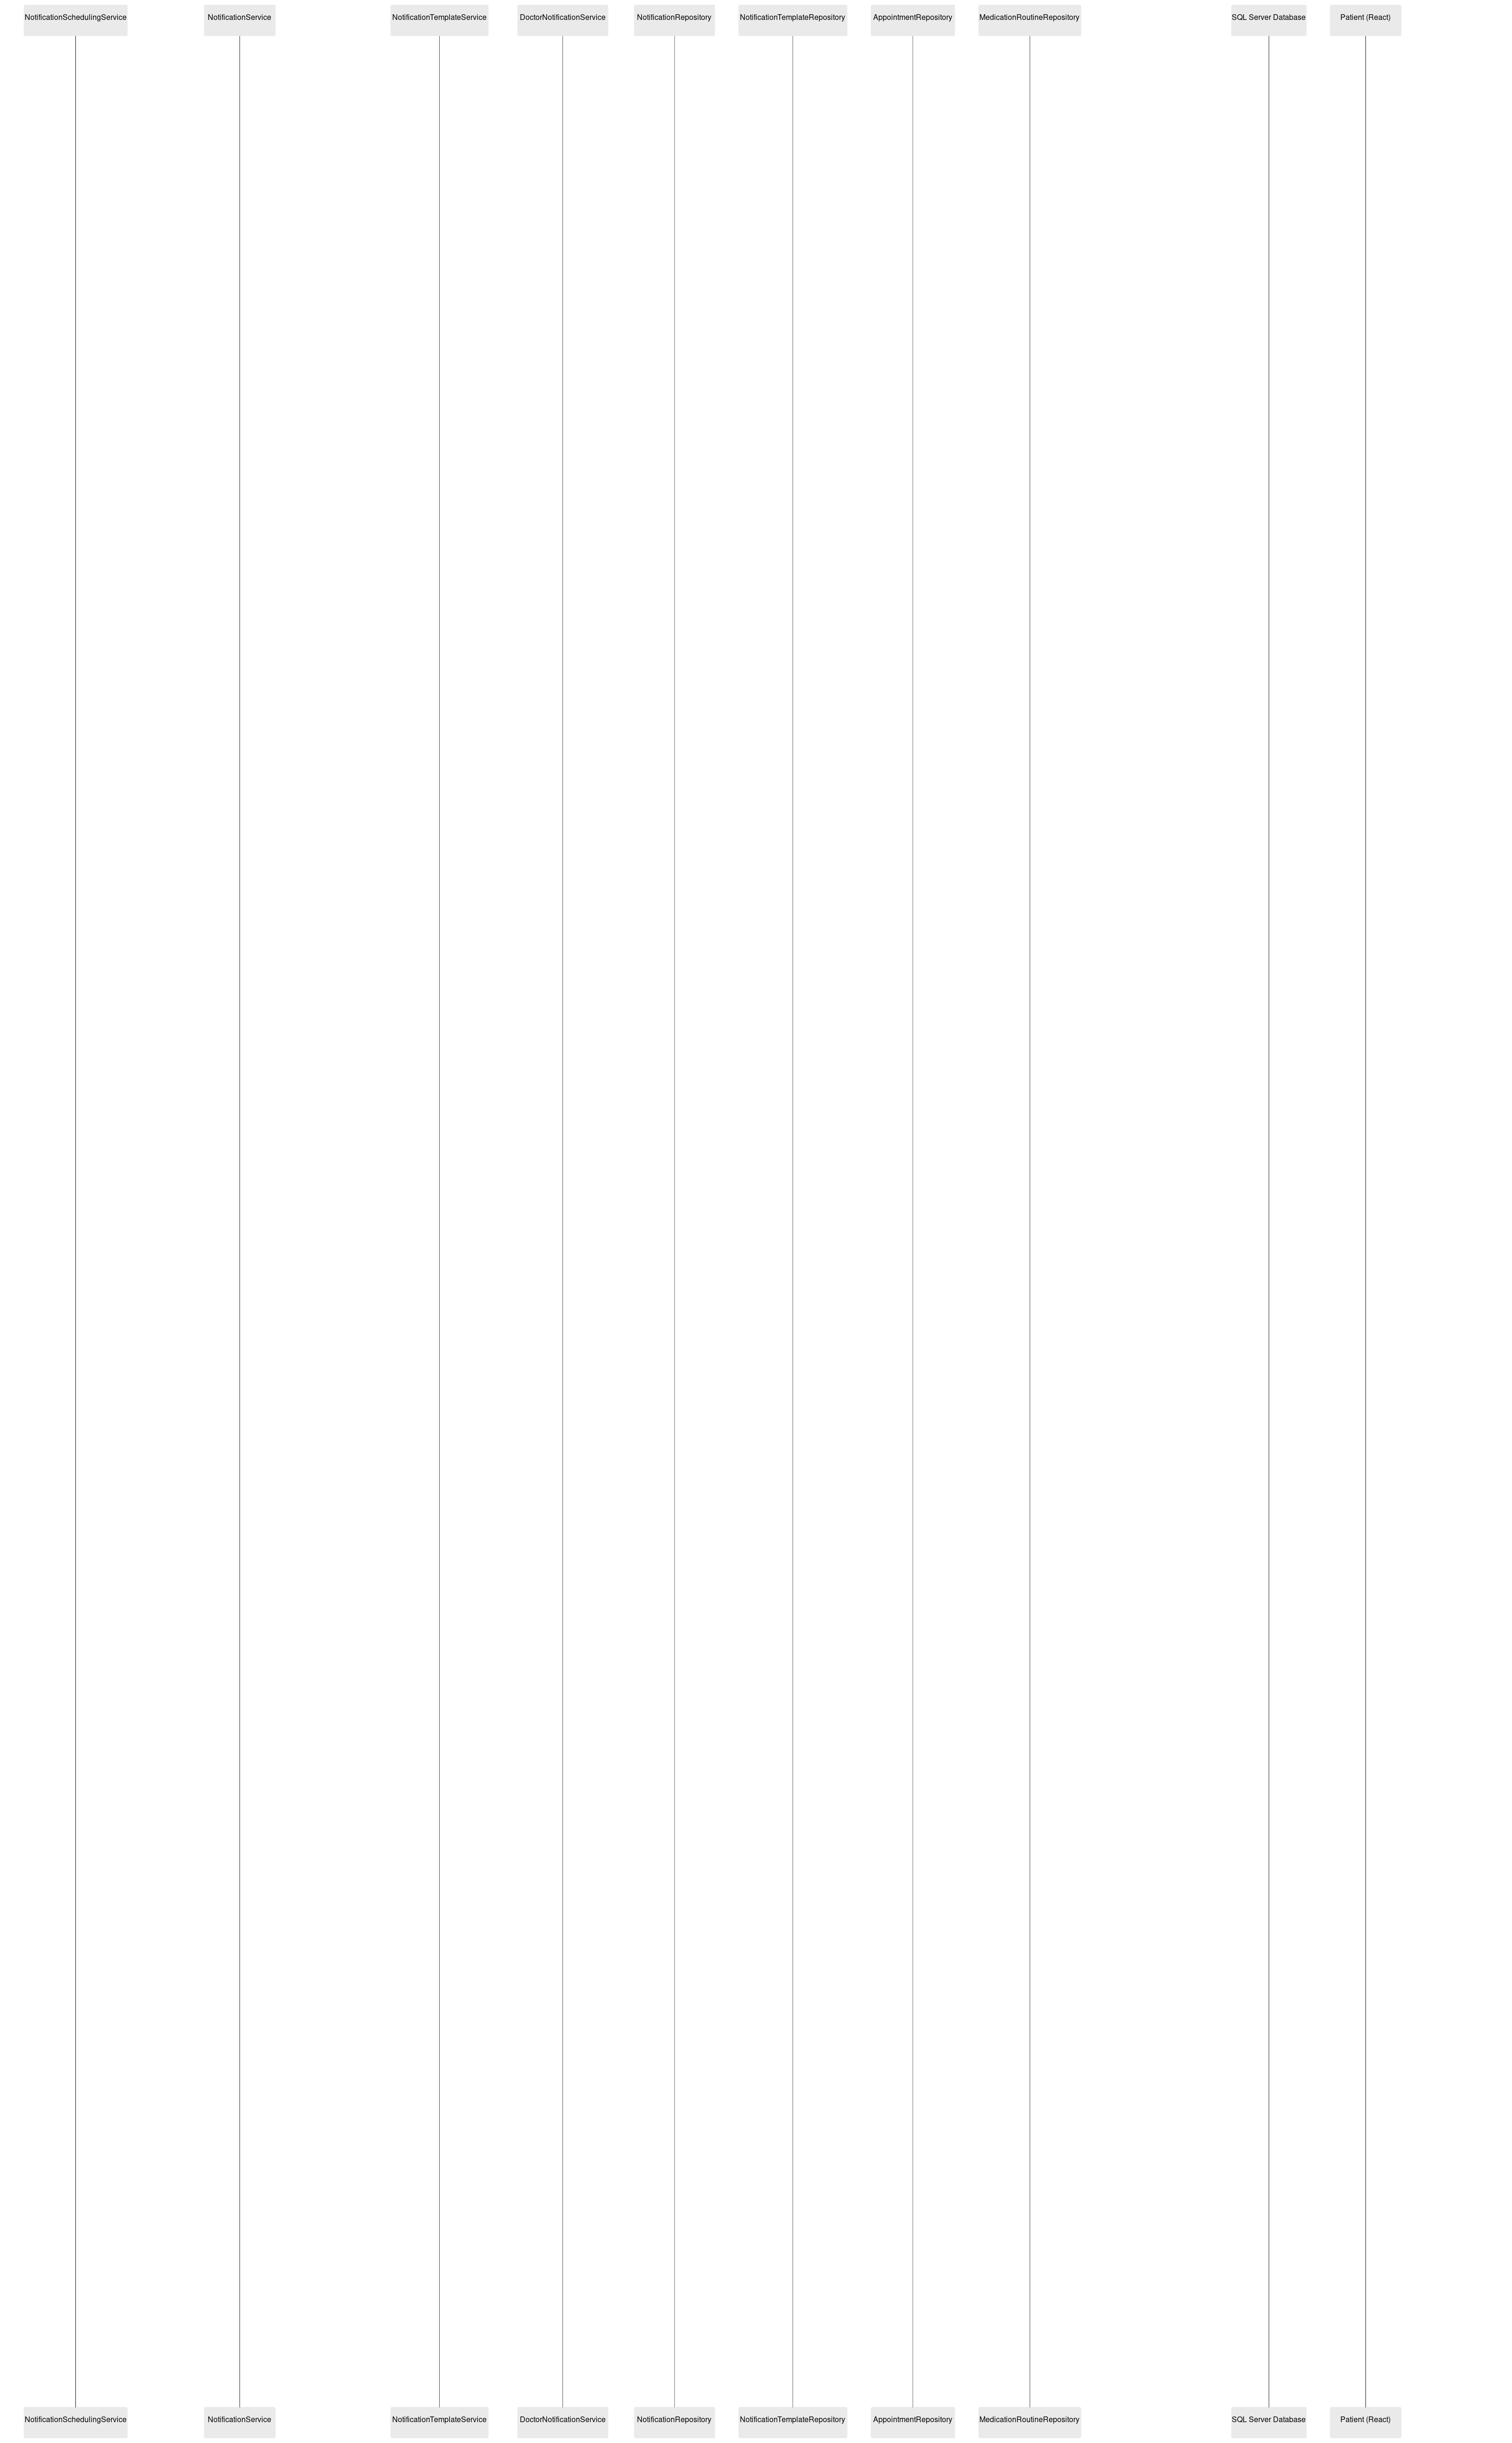
\includegraphics[width=0.9\textwidth]{diagrams/notification_sequence.png}
\caption{Notification Processing Sequence Diagram}
\label{fig:notification-sequence}
\end{figure}

\subsubsection{Database Queries}

\begin{lstlisting}[language=SQL, caption=Notification Management Queries]
-- Create new notification
INSERT INTO Notifications (UserID, Type, Title, Message, Priority, 
                          RelatedEntityID, RelatedEntityType, ScheduledFor, templateId)
VALUES (?, ?, ?, ?, ?, ?, ?, ?, ?);

-- Get user notifications with pagination
SELECT n.*, nt.name as TemplateName 
FROM Notifications n
LEFT JOIN NotificationTemplates nt ON n.templateId = nt.templateId
WHERE n.UserID = ? AND n.IsRead = 0
ORDER BY n.Priority DESC, n.CreatedAt DESC
OFFSET ? ROWS FETCH NEXT ? ROWS ONLY;

-- Schedule appointment reminders
INSERT INTO AppointmentReminders (AppointmentID, PatientUserID, ReminderType, ReminderDateTime)
SELECT AppointmentID, PatientUserID, '24_HOUR', DATEADD(hour, -24, AppointmentDateTime)
FROM Appointments 
WHERE AppointmentDateTime > GETDATE() AND Status = 'Scheduled';

-- Process scheduled notifications
UPDATE Notifications 
SET SentAt = GETDATE(), status = 'SENT'
WHERE ScheduledFor <= GETDATE() AND status = 'PENDING';

-- Mark notification as read
UPDATE Notifications 
SET IsRead = 1, UpdatedAt = GETDATE()
WHERE NotificationID = ? AND UserID = ?;

-- Get notification templates by type
SELECT * FROM NotificationTemplates 
WHERE type = ? AND isActive = 1 
ORDER BY name;

-- Create medication reminder instances
INSERT INTO MedicationReminders (RoutineID, PatientUserID, ReminderDate, ReminderTime)
SELECT RoutineID, PatientUserID, ?, TimeOfDay
FROM MedicationRoutines 
WHERE IsActive = 1 AND ReminderEnabled = 1;
\end{lstlisting}

\subsection{ARV Treatment Management}

This section details the Antiretroviral (ARV) treatment management system for HIV patients.

\subsubsection{Class Diagram}

\begin{figure}[H]
\centering
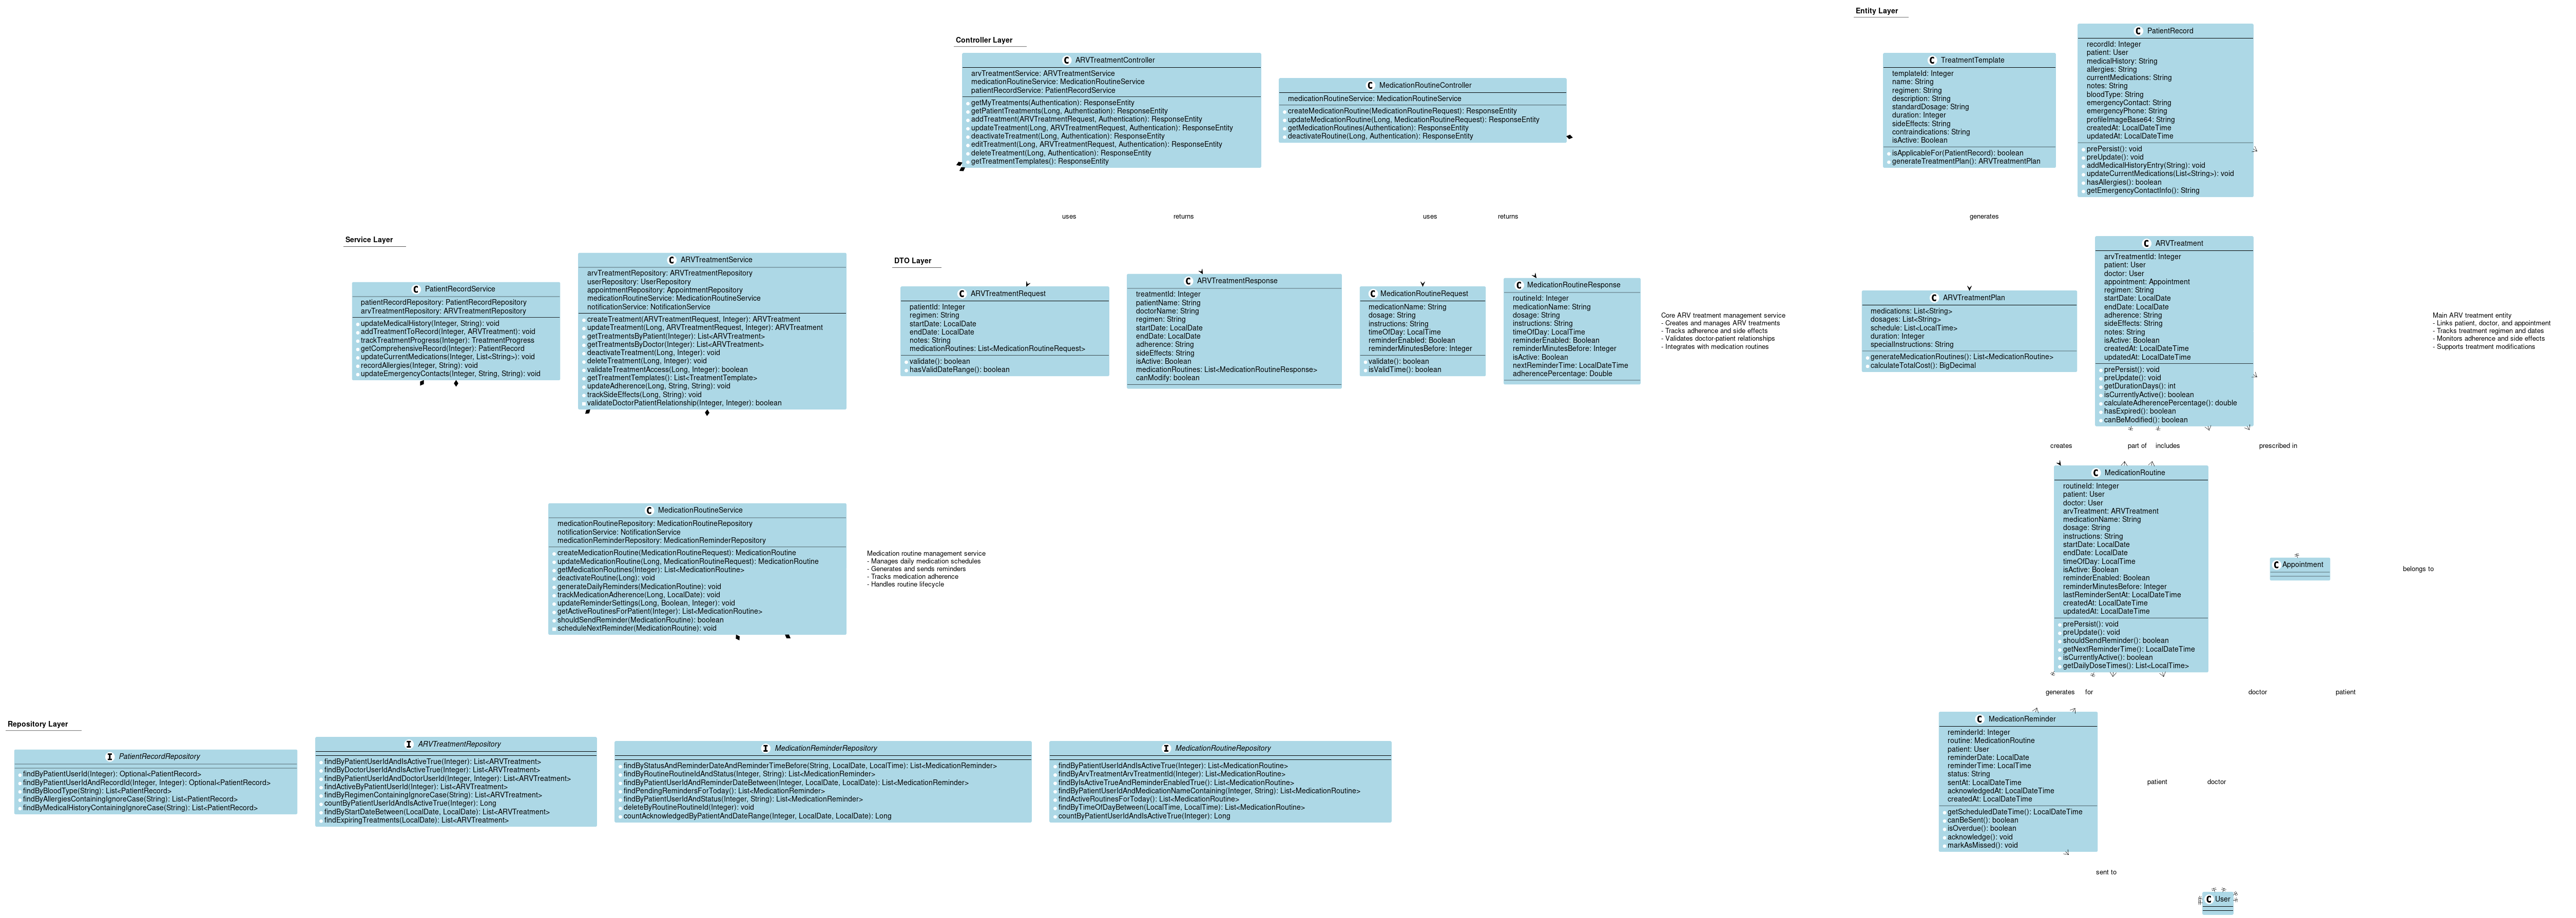
\includegraphics[width=0.9\textwidth]{diagrams/arv_treatment_class_diagram.png}
\caption{ARV Treatment Management Class Diagram}
\label{fig:arv-class-diagram}
\end{figure}

\subsubsection{Class Specifications}

\paragraph{ARVTreatmentController Class}
\begin{longtable}{|c|l|p{8cm}|}
\hline
\textbf{No} & \textbf{Method} & \textbf{Description} \\
\hline
01 & getMyTreatments() & GET /api/arv-treatments/my-treatments - Retrieves ARV treatments for authenticated patient \\
\hline
02 & getPatientTreatments() & GET /api/arv-treatments/patient/\{patientId\} - Retrieves treatments for specific patient (doctor access) \\
\hline
03 & addTreatment() & POST /api/arv-treatments/add - Creates new ARV treatment record \\
\hline
04 & updateTreatment() & PUT /api/arv-treatments/\{treatmentId\} - Updates existing ARV treatment \\
\hline
05 & deactivateTreatment() & PUT /api/arv-treatments/\{treatmentId\}/deactivate - Deactivates treatment (end of regimen) \\
\hline
06 & editTreatment() & PUT /api/arv-treatments/\{treatmentId\}/edit - Edits treatment details and notes \\
\hline
07 & deleteTreatment() & DELETE /api/arv-treatments/\{treatmentId\} - Deletes treatment record \\
\hline
08 & getTreatmentTemplates() & GET /api/arv-treatments/templates - Retrieves standard treatment regimen templates \\
\hline
\end{longtable}

\paragraph{MedicationRoutineService Class}
\begin{longtable}{|c|l|p{8cm}|}
\hline
\textbf{No} & \textbf{Method} & \textbf{Description} \\
\hline
01 & createMedicationRoutine() & Creates new daily medication routine with reminder scheduling \\
\hline
02 & updateMedicationRoutine() & Updates existing medication routine and reschedules reminders \\
\hline
03 & getMedicationRoutines() & Retrieves active medication routines for patient \\
\hline
04 & deactivateRoutine() & Deactivates medication routine when treatment ends \\
\hline
05 & generateDailyReminders() & Generates daily medication reminders based on routine schedule \\
\hline
06 & trackMedicationAdherence() & Tracks medication adherence based on reminder acknowledgments \\
\hline
\end{longtable}

\subsubsection{Sequence Diagram}

\begin{figure}[H]
\centering
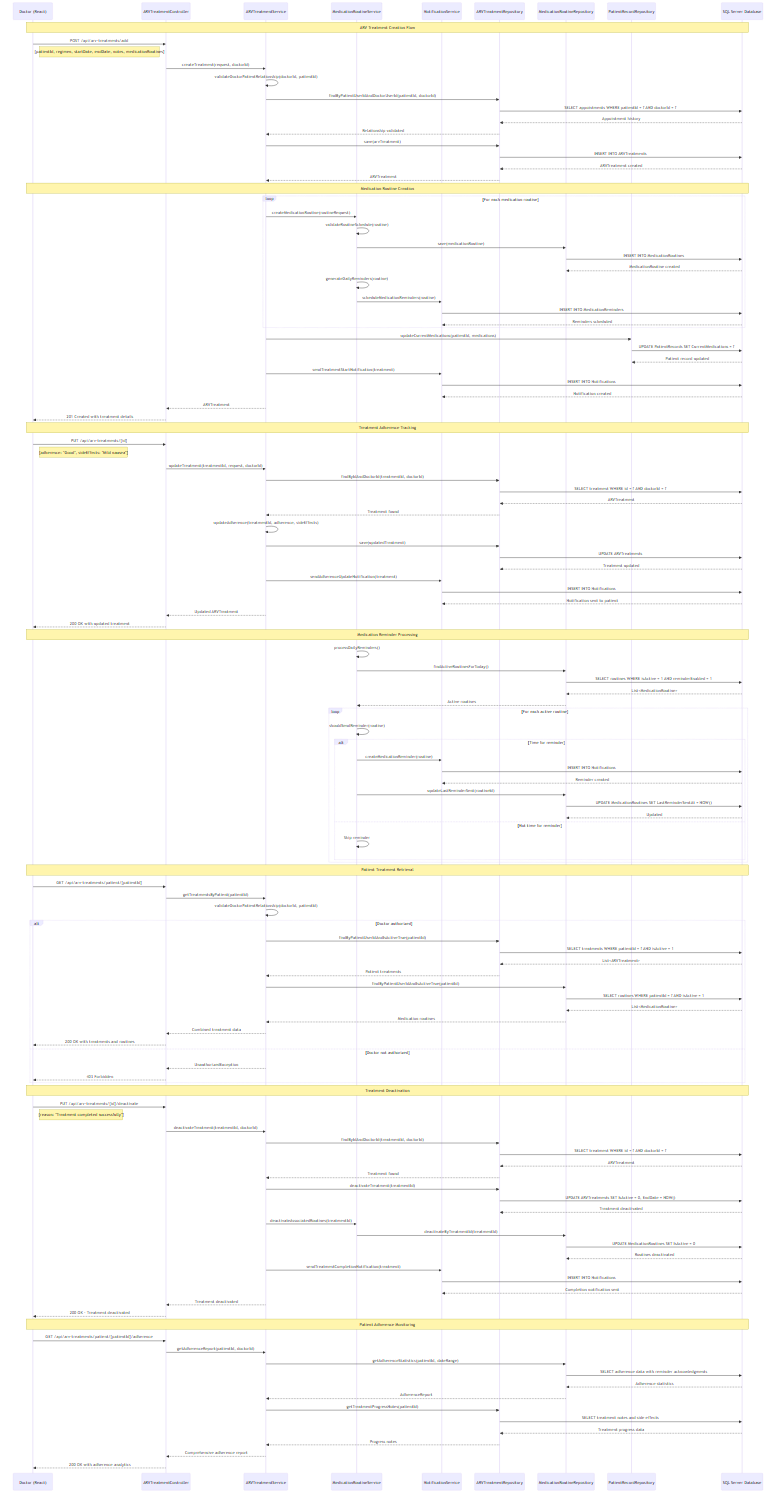
\includegraphics[width=0.9\textwidth]{diagrams/arv_treatment_sequence.png}
\caption{ARV Treatment Creation Sequence Diagram}
\label{fig:arv-sequence}
\end{figure}

\subsubsection{Database Queries}

\begin{lstlisting}[language=SQL, caption=ARV Treatment Management Queries]
-- Create ARV treatment
INSERT INTO ARVTreatments (PatientUserID, DoctorUserID, AppointmentID, 
                          Regimen, StartDate, EndDate, Notes, IsActive)
VALUES (?, ?, ?, ?, ?, ?, ?, 1);

-- Get patient treatments with doctor details
SELECT at.*, d.FirstName as DoctorFirstName, d.LastName as DoctorLastName,
       p.FirstName as PatientFirstName, p.LastName as PatientLastName
FROM ARVTreatments at
INNER JOIN Users du ON at.DoctorUserID = du.UserID
INNER JOIN DoctorProfiles d ON du.UserID = d.UserID
INNER JOIN Users pu ON at.PatientUserID = pu.UserID
INNER JOIN PatientProfiles p ON pu.UserID = p.UserID
WHERE at.PatientUserID = ? AND at.IsActive = 1
ORDER BY at.CreatedAt DESC;

-- Create medication routine
INSERT INTO MedicationRoutines (PatientUserID, DoctorUserID, ARVTreatmentID,
                               MedicationName, Dosage, Instructions, StartDate, 
                               EndDate, TimeOfDay, ReminderEnabled, ReminderMinutesBefore)
VALUES (?, ?, ?, ?, ?, ?, ?, ?, ?, 1, 30);

-- Update treatment adherence
UPDATE ARVTreatments 
SET Adherence = ?, SideEffects = ?, Notes = ?, UpdatedAt = GETDATE()
WHERE ARVTreatmentID = ?;

-- Get active medication routines for reminders
SELECT mr.*, p.FirstName, p.LastName, u.Email
FROM MedicationRoutines mr
INNER JOIN Users u ON mr.PatientUserID = u.UserID
INNER JOIN PatientProfiles p ON u.UserID = p.UserID
WHERE mr.IsActive = 1 AND mr.ReminderEnabled = 1
  AND mr.StartDate <= GETDATE() 
  AND (mr.EndDate IS NULL OR mr.EndDate >= GETDATE());
\end{lstlisting}

\subsection{System Architecture Components}

This section provides an overview of the complete system architecture including frontend-backend integration.

\subsubsection{System Architecture Diagram}

\begin{figure}[H]
\centering
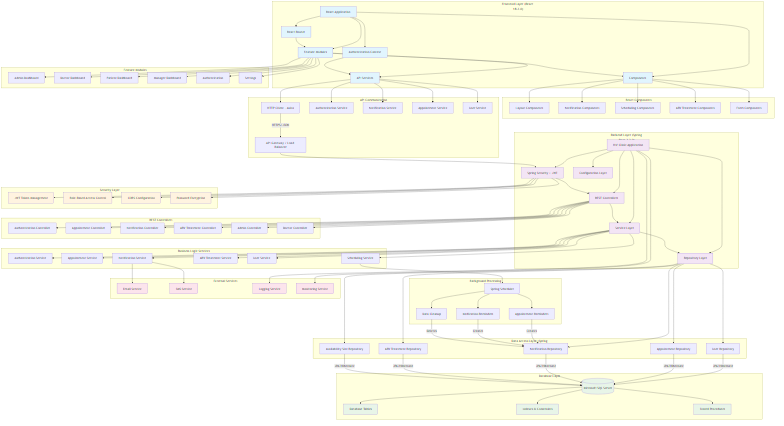
\includegraphics[width=0.9\textwidth]{diagrams/system_architecture.png}
\caption{System Architecture Overview}
\label{fig:system-architecture}
\end{figure}

\subsubsection{Technology Stack}

\begin{table}[H]
\centering
\caption{Technology Stack Components}
\label{tab:tech-stack}
\begin{tabularx}{\textwidth}{|l|l|X|}
\hline
\textbf{Layer} & \textbf{Technology} & \textbf{Description} \\
\hline
Frontend & React 18.2.0 & Modern JavaScript library for building user interfaces with hooks and functional components \\
\hline
Frontend Routing & React Router 6.x & Declarative routing for React applications with nested routes and authentication guards \\
\hline
State Management & React Context API & Built-in state management for authentication and global application state \\
\hline
HTTP Client & Axios & Promise-based HTTP client for API communication with interceptors for authentication \\
\hline
Backend Framework & Spring Boot 3.2.0 & Java-based framework for building enterprise applications with auto-configuration \\
\hline
Security & Spring Security 6.x & Comprehensive security framework with JWT authentication and role-based access control \\
\hline
Data Access & Spring Data JPA & Abstraction layer for database operations with Hibernate ORM \\
\hline
Database & Microsoft SQL Server & Enterprise-grade relational database with T-SQL support \\
\hline
Build Tool & Maven 3.9.x & Project management and build automation tool for Java applications \\
\hline
Java Version & OpenJDK 17 & Long-term support version of Java with modern language features \\
\hline
\end{tabularx}
\end{table}

\subsubsection{Security Architecture}

\begin{table}[H]
\centering
\caption{Security Architecture Components}
\label{tab:security-architecture}
\begin{tabularx}{\textwidth}{|l|X|}
\hline
\textbf{Component} & \textbf{Description} \\
\hline
JWT Authentication & JSON Web Token-based stateless authentication with 24-hour expiration \\
\hline
Role-Based Access Control & Hierarchical role system: Admin > Manager > Doctor > Patient \\
\hline
Password Security & BCrypt hashing with salt for secure password storage \\
\hline
CORS Configuration & Cross-Origin Resource Sharing configuration for frontend-backend communication \\
\hline
Input Validation & Comprehensive input validation using Bean Validation (JSR-303) annotations \\
\hline
SQL Injection Prevention & Parameterized queries and JPA/Hibernate ORM protection \\
\hline
Session Management & Stateless session management with JWT tokens \\
\hline
API Endpoint Security & Method-level security with @PreAuthorize annotations \\
\hline
\end{tabularx}
\end{table}

\subsection{Component Architecture}

\subsubsection{Component Diagram}

\begin{figure}[H]
\centering
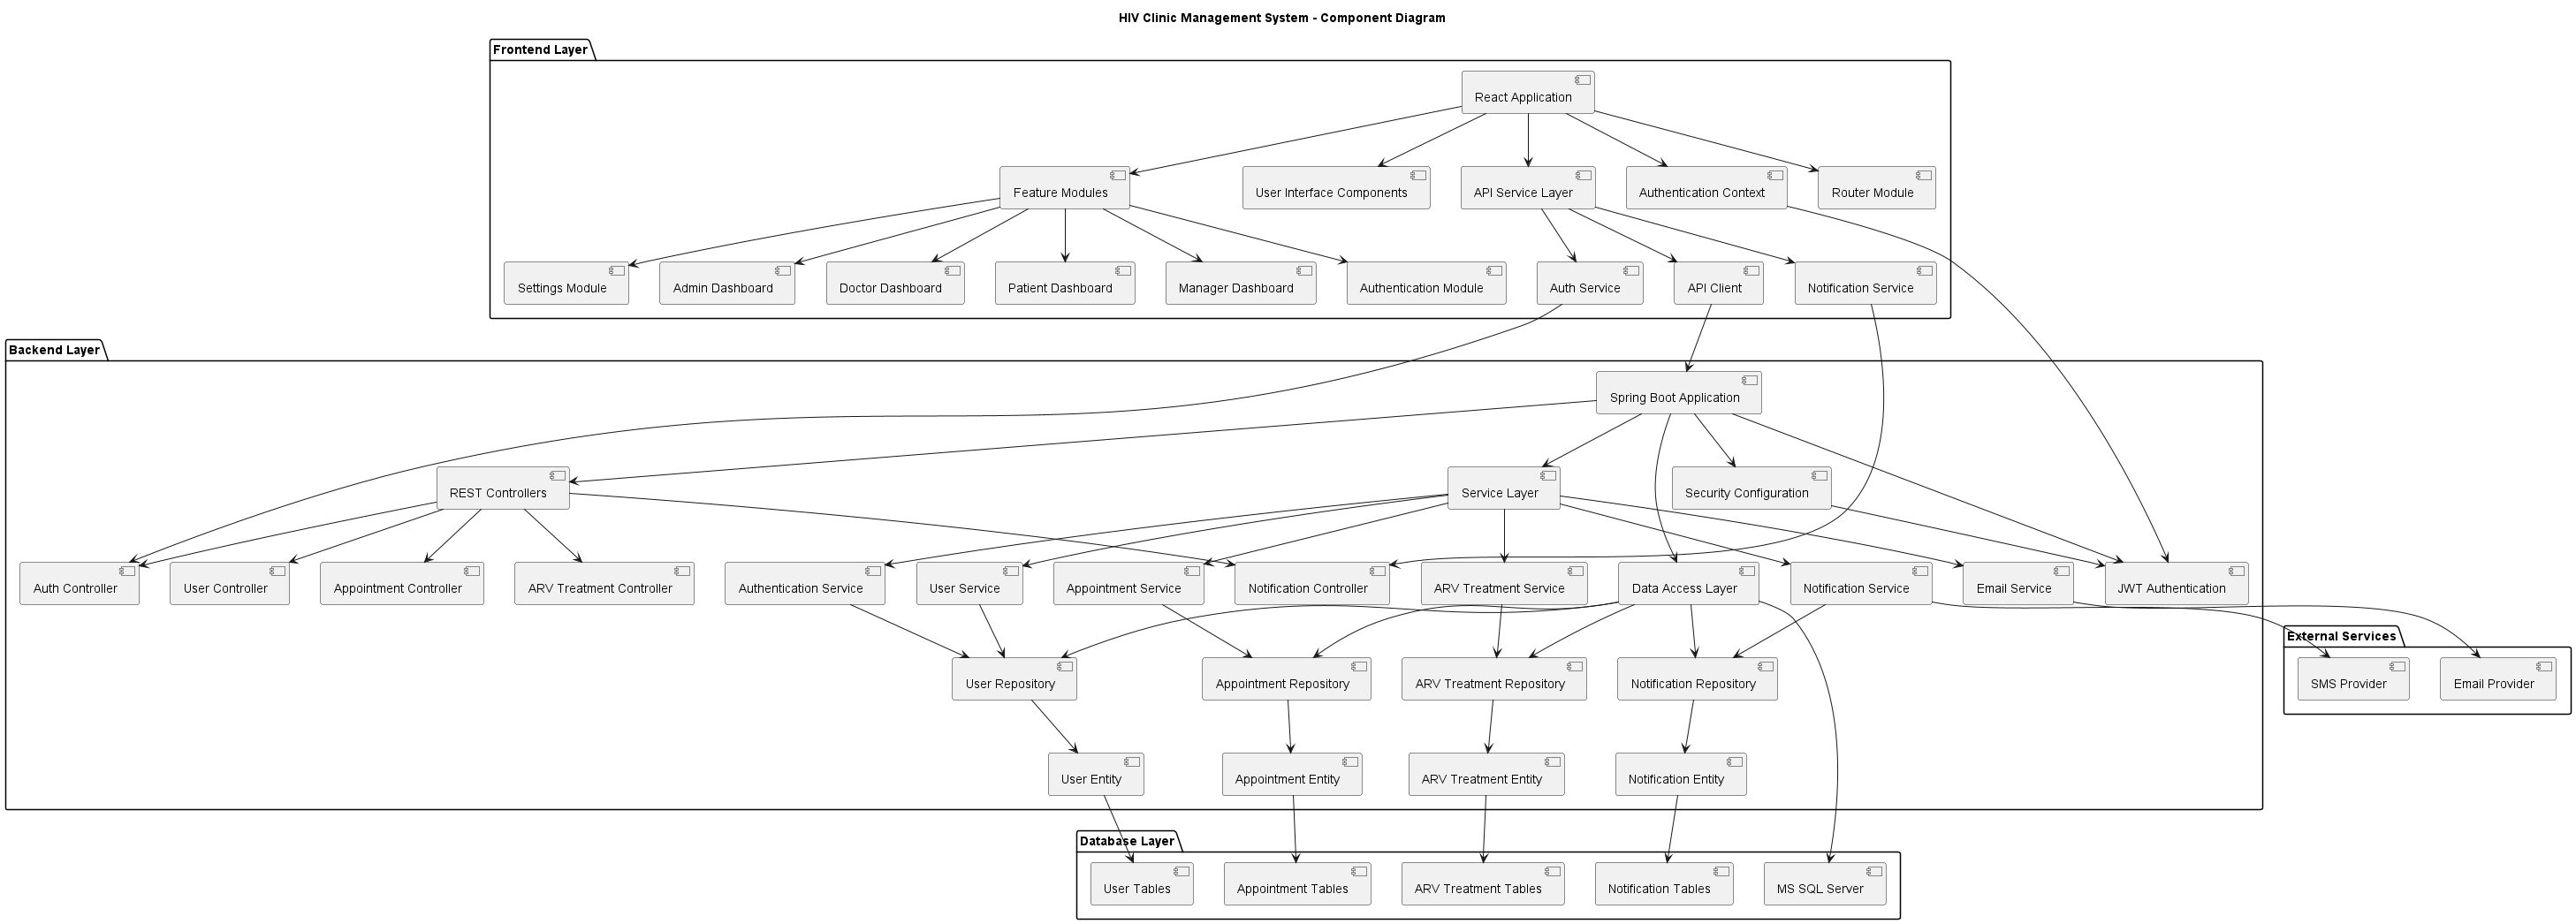
\includegraphics[width=0.9\textwidth]{diagrams/component_diagram.png}
\caption{System Component Architecture}
\label{fig:component-diagram}
\end{figure}

\subsubsection{Deployment Architecture}

\begin{figure}[H]
\centering
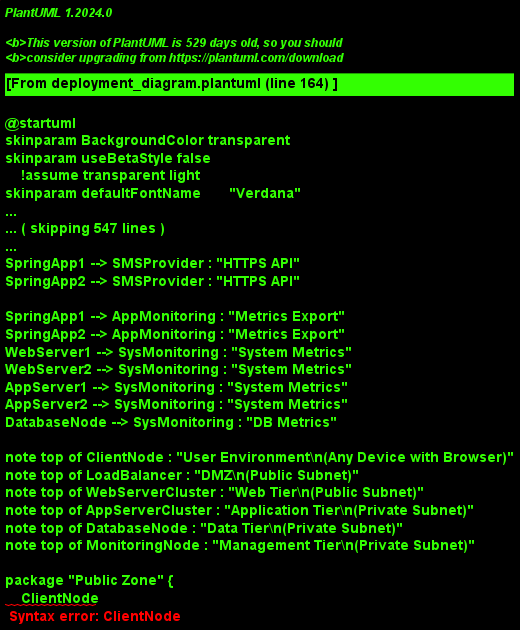
\includegraphics[width=0.9\textwidth]{diagrams/deployment_diagram.png}
\caption{System Deployment Architecture}
\label{fig:deployment-diagram}
\end{figure}

\section{API Documentation}

\subsection{REST API Endpoints}

\begin{longtable}{|l|l|l|p{6cm}|}
\hline
\textbf{Method} & \textbf{Endpoint} & \textbf{Role} & \textbf{Description} \\
\hline
POST & /api/auth/register & Public & User registration with role assignment \\
\hline
POST & /api/auth/login & Public & User authentication and JWT token generation \\
\hline
GET & /api/auth/me & Authenticated & Get current user profile information \\
\hline
PUT & /api/auth/profile & Authenticated & Update user profile information \\
\hline
POST & /api/appointments/book & Patient & Book new appointment with doctor \\
\hline
GET & /api/appointments/patient/my-appointments & Patient & Get patient's appointments \\
\hline
GET & /api/appointments/doctor/my-appointments & Doctor & Get doctor's appointments \\
\hline
PUT & /api/appointments/\{id\}/cancel & Patient/Doctor & Cancel appointment \\
\hline
POST & /api/doctors/availability & Doctor & Create availability slots \\
\hline
GET & /api/doctors/\{id\}/available-slots & Patient & Get doctor's available slots \\
\hline
POST & /api/arv-treatments/add & Doctor & Create ARV treatment record \\
\hline
GET & /api/arv-treatments/my-treatments & Patient & Get patient's ARV treatments \\
\hline
GET & /api/notifications & Authenticated & Get user notifications \\
\hline
POST & /api/notifications/\{id\}/read & Authenticated & Mark notification as read \\
\hline
GET & /api/admin/users & Admin & Get all users (admin only) \\
\hline
POST & /api/admin/doctors & Admin & Create doctor profile \\
\hline
GET & /api/manager/stats & Manager & Get system statistics \\
\hline
\end{longtable}

\section{System Behavior and Network Architecture}

\subsection{State Transition Diagrams}

\begin{figure}[H]
\centering
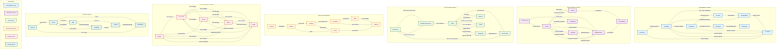
\includegraphics[width=0.9\textwidth]{diagrams/state_transition_diagram.png}
\caption{System State Transition Diagrams}
\label{fig:state-transition-diagram}
\end{figure}

\subsection{Network Architecture}

\begin{figure}[H]
\centering
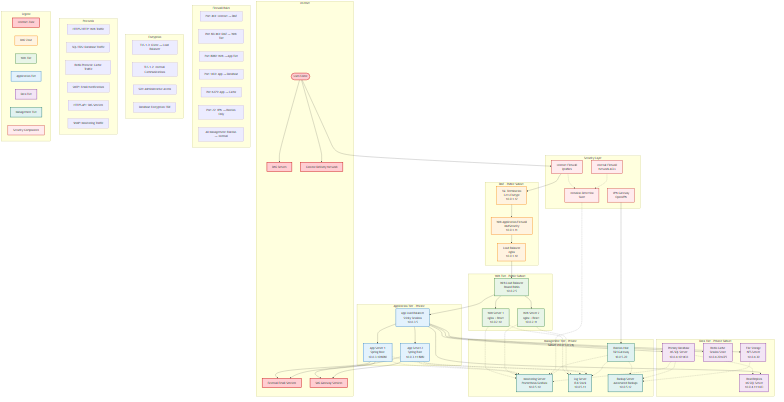
\includegraphics[width=0.9\textwidth]{diagrams/network_architecture.png}
\caption{Network Architectureand Security Zones}
\label{fig:component-diagram}
\end{figure}

\section{Deployment Architecture}

\subsection{Development Environment}

\begin{itemize}
\item \textbf{Frontend Development Server}: Vite development server on port 3000
\item \textbf{Backend Development Server}: Spring Boot embedded Tomcat on port 8080
\item \textbf{Database}: Microsoft SQL Server LocalDB or SQL Server Express
\item \textbf{Build Tools}: Maven for backend, npm/yarn for frontend
\end{itemize}

\subsection{Production Deployment}

\begin{itemize}
\item \textbf{Frontend}: Static files served by Nginx or Apache HTTP Server
\item \textbf{Backend}: Java JAR file deployed on application server (Tomcat, Jetty)
\item \textbf{Database}: Microsoft SQL Server Standard/Enterprise Edition
\item \textbf{Security}: HTTPS with SSL/TLS certificates
\item \textbf{Monitoring}: Application logging with logback and system monitoring
\end{itemize}

\section{Conclusion}

The HIV Clinic Management System implements a comprehensive, secure, and scalable solution for managing HIV patient care. The system architecture follows modern software engineering principles with clear separation of concerns, robust security measures, and comprehensive data management capabilities.

Key architectural strengths include:
\begin{itemize}
\item \textbf{Layered Architecture}: Clean separation between presentation, business logic, and data access layers
\item \textbf{Security-First Design}: Comprehensive security implementation with JWT authentication and role-based access control
\item \textbf{Scalable Database Design}: Normalized database schema with proper indexing and referential integrity
\item \textbf{RESTful API Design}: Well-designed REST API with consistent naming conventions and proper HTTP methods
\item \textbf{Comprehensive Notification System}: Automated notification system for appointments and medication reminders
\item \textbf{Audit Trail}: Complete audit trail for all critical operations and data changes
\end{itemize}

The system is designed to be maintainable, extensible, and capable of handling future enhancements while maintaining data integrity and security standards required for healthcare applications.

\end{document}